\documentclass{sig-alternate-05-2015}

\usepackage{hyperref}
 \hypersetup{
    colorlinks=true,
    linkcolor=black,
    citecolor=black,
    filecolor=magenta,
    urlcolor=blue
}
\usepackage{pifont} % for \fleur macro
\usepackage[T1]{fontenc}
\usepackage[utf8x]{inputenc}
\usepackage{url}
\usepackage{array}
\usepackage{infer}
\usepackage{listings}
\usepackage{xspace}
\usepackage{amsmath}
\usepackage{stmaryrd}
\usepackage{tikz}
\usepackage{xcolor}
\usepackage{alltt}
\usepackage{subcaption}
\usepackage{balance}

\definecolor{darkergray}{gray}{0.38}

\usepackage{lstcoq}
\lstset{language=Coq,%
   % basicstyle=\ttfamily,%
   % keywordstyle=\color{blue}\ttfamily,%
   columns=fullflexible,%
   moredelim=[is][\itshape]{\#}{\#},%
   showstringspaces=false,%
}
\lstnewenvironment{lstcoq}%
{\footnotesize \lstset{language=Coq,keepspaces=true}}
{}

\setlength{\pdfpagewidth}{8.5in}
\setlength{\pdfpageheight}{11in}

%\pagenumbering{arabic}

%%%%%%
%%%%%% Hyperlinks to code
\newcommand{\HTMLBase}{https://querycert.github.io}
\newcommand{\coqHTMLBase}{\HTMLBase/sigmod17}
\newcommand{\coqBaseModule}{Qcert.}
\newcommand{\projectname}{Q*cert}
%%%%%%
%%%%%%

%% Macros used in the paper

\newcommand{\anonymize}[2]{#2}

\newcommand{\coqHTMLBase}{https://querycert.github.io/icfp17}
% \newcommand{\coqHTMLBase}{file:///Users/lmandel/Desktop/qcert}
% \newcommand{\coqBaseModule}{doc/Qcert}
\newcommand{\coqBaseModule}{doc}
% \newcommand{\coqBaseModule}{html/Qcert}
% \newcommand{\coqurl}[3]{\coqHTMLBase/\coqBaseModule.#1.#2.html\##3}
\newcommand{\coqurl}[3]{\coqHTMLBase/\coqBaseModule/#2.html\##3}
\newcommand{\projectname}{Q*cert}

\newcommand{\fleur}{\ding{95}}
\newcommand{\coqtop}{{\href{\coqHTMLBase}{\fleur}}\xspace}
% \newcommand{\coqdef}[2]{{\href{\coqHTMLBase/\coqBaseModule.#1\##2}{\fleur}}\xspace}
\newcommand{\coqdef}[3]{{\href{\coqurl{#1}{#2}{#3}}{\fleur}}\xspace}

\newcommand{\NRAEnv}{\texorpdfstring{NRA$^{\!\mbox{\it e}}$}{NRAe}\xspace}
\newcommand{\NRALambda}{\texorpdfstring{NRA$^{\lambda}$}{NRAλ}\xspace}


%% Colors
\definecolor{darkred}{rgb}{0.55, 0.0, 0.0}

%%% textalltt

\makeatletter
\newcommand*{\textalltt}{}
\DeclareRobustCommand*{\textalltt}{%
  \begingroup
    \let\do\@makeother
    \dospecials
    \catcode`\\=\z@
    \catcode`\{=\@ne
    \catcode`\}=\tw@
    \verbatim@font\@noligs
    \@vobeyspaces
    \frenchspacing
    \@textalltt
}
\newcommand*{\@textalltt}[1]{%
    #1%
  \endgroup
}
\makeatother


%%% ODM
\newcommand{\textblue}[1]{{\color{blue}{#1}}}
\newcommand{\textred}[1]{{\color{darkred}{#1}}}
\newcommand{\odmkw}[1]{\textblue{\textit{#1}}}
\newcommand{\odmagg}[1]{{\color{darkred}{#1}}}

\lstdefinelanguage{jrules}{
  keywords={aggregate,do,emit,false,groupby,insert,new,rule,then,true,update,when},
  numbers=none, columns=flexible, captionpos=b,
  basicstyle={\small\selectfont\ttfamily}, keywordstyle=\bfseries,
  morecomment=[l]{//},
  morecomment=[s]{/*}{*/},
  xleftmargin=0.5cm,
  abovecaptionskip=0em,
  belowcaptionskip=0em
% ,frame=tlbr,framesep=4pt,framerule=0pt
}


%%% Local Variables:
%%% mode: latex
%%% TeX-master: "icfp17"
%%% End:


\CopyrightYear{2017}
\setcopyright{acmcopyright}
\conferenceinfo{SIGMOD'17,}{May 14-19, 2017, Chicago, Illinois, USA}
\isbn{978-1-4503-4197-4/17/05}\acmPrice{\$15.00}
\doi{http://dx.doi.org/10.1145/3035918.3035961}

\clubpenalty=10000 
\widowpenalty = 10000

%% End for macros used in the paper

% Author macros::begin %%%%%%%%%%%%%%%%%%%%%%%%%%%%%%%%%%%%%%%%%%%%%%%%
\title{Handling Environments in a Nested Relational Algebra with Combinators and an Implementation in a Verified Query Compiler}

\numberofauthors{1}
\author{\alignauthor
Joshua S. Auerbach, Martin Hirzel, Louis Mandel,\\Avraham Shinnar \& J\'{e}r\^{o}me Sim\'{e}on\\
       \affaddr{IBM Research}\\
       \affaddr{1101 Kitchawan Rd}\\
       \affaddr{Yorktown Heights, NY 10598}\\
% 2nd. author
}

% Author macros::end %%%%%%%%%%%%%%%%%%%%%%%%%%%%%%%%%%%%%%%%%%%%%%%%%

\begin{document}

\maketitle

\begin{abstract}
  Algebras based on combinators, i.e., variable-free, have been
  proposed as a better representation for query compilation and
  optimization. A key benefit of combinators is that they avoid the
  need to handle variable shadowing or accidental capture during
  rewrites. This simplifies both the optimizer specification and its
  correctness analysis, but the environment from the source language
  has to be reified as records, which can lead to more complex query
  plans.

  This paper proposes \NRAEnv, an extension of a combinators-based
  nested relational algebra (NRA) with built-in support for
  environments. We show that it can naturally encode an equivalent NRA
  with lambda terms and that all optimizations on NRA carry over to
  \NRAEnv. This extension provides an elegant way to represent views
  in query plans, and can radically simplify compilation and
  optimization for source languages with rich environment
  manipulations.
  
  We have specified a query compiler using the Coq proof assistant
  with \NRAEnv at its heart. Most of the compiler, including the query
  optimizer, is accompanied by a (machine-checked) correctness
  proof. The implementation is automatically extracted from the
  specification, resulting in a query compiler with a verified core.
\end{abstract}

\section{Introduction}
\label{sec:introduction}

Some recent development around query languages and query processing is
happening outside traditional database management systems, e.g.,
language-integrated queries~\cite{cooper2007links,Meijer11},
large-scale distributed processing
infrastructure~\cite{armbrust2015spark,BeyerEGBEKOS11-full,OlstonRSKT08},
NoSQL databases~\cite{OngPV14}, or domain specific
languages~\cite{ShinnarSH15}. Understanding and guaranteeing
correctness properties for those new data processing capabilities can
be important when dealing with business critical or personal data. In
relational systems, rule-based optimizers and optimizer
generators~\cite{CareyDFGRSM91,cherniack1996rule,CherniackZ98,FegarasMS93,LeungMSVVZ93,PiraheshHH92}
contribute to the high levels of performance and correctness
confidence by enabling the specification, verification, and
implementation of query compilers. This paper proposes to leverage
modern theorem proving technology as a foundation for building
well-specified and formally verified query compilers.

Although our motivation stems from new query compilation scenarios,
and specifically the extension of a rule-based language with a query
DSL, we believe the approach can be applied in more traditional
database contexts. As was shown in compilers for language integrated
queries~\cite{grust2009ferry}, relying on traditional database
algebras can bring numerous benefits. We follow a similar strategy and
build on top of the nested relational algebra
(NRA)~\cite{CluetM93,fegaras2000optimizing} which has been
successfully used for building query compilers for nested data models,
notably for OQL and XQuery~\cite{MayHM04,re2006complete}.

As observed in prior work~\cite{cherniack1996rule,CherniackZ98},
ensuring correctness remains hard even with a rule-based approach, and
we have encountered similar challenges. Three of the main challenges
are (i)~reasoning about scoping when variables are involved as part of
the optimization rules, (ii)~providing tools to facilitate reasoning
and correctness checking, and (iii)~handling code fragments as part of
the rules. Although most of the previously proposed techniques and
optimizations for NRA directly apply, those three challenges require
special care and are the focus of this paper.

\paragraph*{Handling Environments}

The first challenge is intrinsically difficult for any
compiler\footnote{Proper handling of variable scoping is known as one
  of the main difficulties in solving the POPLmark
  challenge~\cite{AydemirBFFPSVWWZ05}.} and is the central focus of
the paper. Combinator-based
algebras~\cite{cherniack1996rule,ShinnarSH15} have been used to
eliminate variables in an attempt to facilitate reasoning.  However,
they force the query translator to reify environments as part of the
data being processed, which can result in larger and more complex
query plans.

This paper proposes \NRAEnv, an extension to a combinator-based nested
relational algebra with native support for environments.  It avoids
blow-ups in query plan size while facilitating correctness
reasoning. This extension is conservative in the sense that existing
NRA optimizations can be applied even to query plans containing the
new constructs.

\paragraph*{A Verified Query Compiler}

To address the second challenge, we are developing a query compiler
using the Coq proof assistant~\cite{coq} which we use for both the
compiler specification and correctness proofs. A Coq feature called
\emph{extraction}~\cite{coq:extraction} can then be used to
automatically generate the query compiler's code from that
specification.
%
Let us first illustrate the use of Coq for the implementation and
verification of a simple algebraic rewrite. Throughout the paper, we
will use the flower symbol~\coqtop\ to provide hyperlinks to the
corresponding source code.

As in rule-based optimizer generators, optimizations can be written in
Coq as rewrites on algebraic terms. As an example, here is the Coq
code for pushing down a selection operator over a union
operator~(based on the classic distributivity law:
${\qselect{q_0}{q_1 \cup q_2} \equiv \qselect{q_0}{q_1} \cup
  {\qselect{q_0}{q_2}}}$):

\begin{lstcoq}
  Definition select_union_distr_fun q := $\mbox{\hspace*{2cm}\coqdef{NRAEnv.Optim.NRAEnvOptimizer}{select_union_distr_fun}}$
    match q with
    | NRAEnvSelect q0 (NRAEnvBinop AUnion q1 q2) =>
        NRAEnvBinop AUnion (NRAEnvSelect q0 q1)
                           (NRAEnvSelect q0 q2)
    | _ => q
    end.
\end{lstcoq}
This code is written in a functional style and defines a function with
name \coqe{select_union_distr_fun} and one parameter \coqe{q} (the
algebraic plan). The body of the function uses pattern matching to
check whether the terms in \coqe{q} are indeed a selection over an
union, in which case it applies the rewrite, or not, in which case it
leaves the plan unchanged.
%
A key difference with most rule-based optimizer generators, is that
Coq allows the query compiler developer to state (and also prove) the
correctness of this rewrite:

\begin{lstcoq}
  Proposition select_union_distr_fun_correctness q: $\mbox{\hspace*{0.4cm}\coqdef{NRAEnv.Optim.NRAEnvOptimizer}{select_union_distr_fun_correctness}}$
    select_union_distr_fun q ⇒ q.
  Proof.
    tprove_correctness p.
    apply tselect_union_distr.
  Qed.
\end{lstcoq}
This proposition states that for all query plans \coqe+q+, applying
the function \coqe+tselect_union_distr_fun+ returns an equivalent
query. Here the symbol \coqe+⇒+ denotes a notion of type-preserving
equivalence which is used throughout our optimizer and is formally
defined later in the paper.
%
The proposition statement is followed by a proof script that is
mechanically checked. The proof relies on an automated proof tactic
\coqe+tprove_correctness+ which eliminates all trivial cases except
the important one which is solved using the lemma
\coqe+tselect_union_distr+.
%
That lemma itself is simply a type preserving variant of the
distributivity law for selection over union which we saw earlier:

\begin{lstcoq}[mathescape=true]
  Lemma tselect_union_distr q$\sb{0}$ q$\sb{1}$ q$\sb{2}$ : $\mbox{\hspace*{2.4cm}\coqdef{NRAEnv.Optim.TNRAEnvRewrite}{tselect_union_distr}}$
    $\sigma$⟨ q$\sb{0}$ ⟩(q$\sb{1}$ ∪ q$\sb{2}$) ⇒ $\sigma$⟨ q$\sb{0}$ ⟩(q$\sb{1}$) ∪ $\sigma$⟨ q$\sb{0}$ ⟩(q$\sb{2}$).
  Proof. ... Qed.
\end{lstcoq}

Formal verification techniques have been applied to the formalization
of relational~\cite{BenzakenCD14,MalechaMSW10} and
non-relational~\cite{CheneyU11,ShinnarSH15} query languages, but have
seldom been used with query compilers implementation in mind. A
notable exception is the Coko-Kola
project~\cite{cherniack1996rule,CherniackZ98} which relied on the
Larch~\cite{Larch89} theorem prover. Using Coq allowed us to apply
those techniques beyond the query optimizer and prove correct a large
subset of the compilation pipeline, including translations between
intermediate languages and type checking.

\paragraph*{Code Fragments}

The third challenge is handling the need for code fragments as
preconditions for rewrites. Here, we simply take advantage of the
expressive specification language that Coq provides and which can be
used to specify and reason about complex conditions (type conditions,
ordering conditions, etc.) on the algebraic plans. Take for example
the distinct elimination law:

\begin{lstcoq}[mathescape=true]
  Lemma tdup_elim q : nodupA q -> $\sharp$distinct(q) ⇒ q. $\mbox{\hspace*{0.3cm}\coqdef{NRAEnv.Optim.TNRAEnvRewrite}{tdup_elim}}$
  Proof. ... Qed.
\end{lstcoq}

The predicate \coqe{nodupA q} holds when the query plan \coqe{q}
always returns a collection without duplicates, and \coqe+->+ is the
syntax for logical implication in Coq. In contrast to traditional
rule-based optimizers, the \coqe{nodupA} predicate is not a
subroutine written in a traditional programming language but is
written in Coq itself and has also been proved correct.

\paragraph*{Overview}

The next section illustrates the distinction between variable-based
and combinator-based algebras, how that distinction impacts algebraic
equivalences, and introduces \NRAEnv through examples. The rest of the
paper contains the formal treatment for the proposed NRA extension and
its properties, applications, and implementation. This paper makes the
following main contributions:
\begin{itemize}
\item It describes a new approach to handling environments in database
  algebras and defines \NRAEnv, an extension of a combinator-based
  nested relational algebra with support for environments
  (Section~\ref{sec:nraenv}).
\item It extends the traditional notion of algebraic equivalence for
  \NRAEnv and defines algebraic rewrites for environment
  manipulation. A main result is that all existing algebraic
  equivalences for the original combinator-based NRA can be lifted
  ``as is'' to \NRAEnv (Section~\ref{sec:optimization}).
\item It shows that \NRAEnv\ can be effectively compiled back to
  traditional NRA and calculus. This confirms that \NRAEnv has the
  expected expressiveness and provides a bridge for integration into
  existing systems (Section~\ref{sec:export}).
\item It illustrates \NRAEnv on several use cases. We show it can
  naturally encode an equivalent NRA with lambda terms. We also show
  how environment operators provide an elegant way to represent view
  declarations in SQL or OQL~(Section~\ref{sec:queries}). Finally, we
  used \NRAEnv\ to radically simplify optimization for a query DSL
  built on top of JRules~\cite{jrules-book}~(Section~\ref{sec:rules}).
\end{itemize}

There is more to a query compiler than its core algebra and
optimizer. In Section~\ref{section:implementation}, we report on the
status of our effort in building Q*cert, an end-to-end, formally
verified, query compiler based on \NRAEnv. We review aspects that were
left out of the main formal treatment in the paper, notably: front-end
support, code generation, type checking and handling of user-defined
types and functions.

Although not necessary to follow the paper, the reader can consult the
full compiler specification which we have made available at
\url{https://querycert.github.io/sigmod17}.
%

%%% Local Variables:
%%% TeX-master: "main"
%%% End:


\section{Variables Revisited}
\label{sec:variables}

\begin{figure*}
  \begin{center}
\begin{subfigure}[b]{0.95\linewidth}
\centering
    \begin{minipage}{0.9\linewidth}
      \centering
      \[\begin{array}{l@{\ }r@{\ \equiv\ }l}
        \textbf{T1 (lambdas):~} & \lmapop(\llambda{a}{a.\mathit{city}})(\lmapop(\llambda{p}{p.\mathit{addr}})(P)) & \lmapop(\llambda{p}{(p.\mathit{addr}).\mathit{city}})(P)\\
        \textbf{T1$^c$ (combin.):~} & \qmap{\qID.\mathit{a}.\mathit{city}}{\qmap{[a:\qID]}{\qmap{\qID.\mathit{p}.\mathit{addr}}{\qmap{[p:\qID]}{P}}}} & \qmap{\qID.\mathit{p}.\mathit{addr}.\mathit{city}}{\qmap{[p:\qID]}{P}}\\
        \textbf{T1$^e$ (\NRAEnv):~} & \qmap{\qENV.\mathit{a}.\mathit{city}\;\circ^e\;[a:\qID]}{\qmap{\qENV.\mathit{p}.\mathit{addr}\;\circ^e\;[p:\qID]}{P}} & \qmap{\qENV.\mathit{p}.\mathit{addr}.\mathit{city}\;\circ^e\;[p:\qID]}{P}\\
      \end{array}\]
    \end{minipage}
  \end{subfigure}
\begin{subfigure}[b]{0.95\linewidth}
\centering
    \begin{minipage}{0.9\linewidth}
      \centering
      \[\begin{array}{l@{\ }l}
      \textbf{A4 (lambdas):~} & \lmapop(\llambda{p}{[ \mathit{person}: p,\;\mathit{kids}: \lselop(\llambda{c}{p.\mathit{age} > 25})(p.\mathit{child}) ]}(P)\\
      \textbf{A4$^c$ (combin.):~} & \qmap{\Big[\textstyle \mathit{person}: \qID.p,\;\mathit{kids}: \qselect{\qID.p.\mathit{age} > 25}{\qdjoin{\qmap{[c:\qID]}{\qID.p.\mathit{child}}}{\{\qID\}}} \Big]}{\qmap{[p:\qID]}{P}}\\
      \textbf{A4$^e$ (\NRAEnv):~} & \qmap{\textstyle [ \mathit{person}: \qENV.p,\;\mathit{kids}: \qselect{(\qENV.p.\mathit{age} > 25)\;\circ^e\;(\qENV \oplus [c:\qID])}{\qENV.p.\mathit{child}} ]\;\circ^e\;[p:\qID]}{P}
      \end{array}\]
    \end{minipage}
  \end{subfigure}
  \end{center}
  \caption{Three styles of nested relational algebra for \textbf{T1} and \textbf{A4} (Examples from Cherniack and Zdonik~\cite{cherniack1996rule})}
  \label{figure:threenras}
\end{figure*}

The treatment of variables and scoping in compilers is notoriously
challenging, and a wide range of techniques have been proposed to
encode variables in a way that facilitates reasoning, either for
correctness or optimization purposes~\cite{AydemirBFFPSVWWZ05}. The
topic has received less attention in the database context. One area
where issues related to variable handling come to the fore is
rule-based
optimizers~\cite{CareyDFGRSM91,cherniack1996rule,CherniackZ98,FegarasMS93,LeungMSVVZ93,PiraheshHH92}.
Cherniack and Zdonik clearly describe the challenges caused by
variables in database algebras and propose a solution based on
combinators~\cite{cherniack1996rule}. Figure~\ref{figure:threenras}
shows two examples from that paper. We use $e.a$ (resp.\ $[a_1:e_1,
  \ldots, a_n:e_n]$) to denote record access (resp.\ record
construction).

\paragraph*{Lambdas vs. Combinators}

Most internal database algebras support some form of explicit binders,
most commonly expressed as
lambdas~\cite{CareyDFGRSM91,cherniack1996rule,FegarasMS93}.  Example
\textbf{T1} in Figure~\ref{figure:threenras} shows an equivalence
written in AQUA~\cite{LeungMSVVZ93} that illustrates how lambdas are
used inside iterators with \lmapop\ (resp.\ \lselop) corresponding to
functional map (resp.\ selection).

Both query plans in \textbf{T1} return the content of the city fields
within the addr fields in the records returned by~$P$. The rewrite is
a classic loop fusion: in lambda form, it can be expressed using
beta-reduction (or capture avoiding substitution) as suggested by
Fegaras et al.~\cite{FegarasMS93}:
\begin{align*}
  \lmapop(\llambda{x}{e})(\lmapop(\llambda{y}{u})(v)) \equiv \lmapop(\llambda{y}{e[u/x]})(v)
\end{align*}

Although techniques exist (e.g.,~\cite{abadi1991explicit}) to
implement or reason about binders and support such substitutions
effectively, most of them remain challenging to mechanize and prove
correct~\cite{AydemirBFFPSVWWZ05}. As Cherniack and Zdonik first
pointed out~\cite{cherniack1996rule}, it is also unnecessarily complex
in the database context as equivalent combinator-based algebras can
avoid binders and variables. We use Cluet and Moerkotte's
algebra~\cite{CluetM93} as our starting point, because (i) it has been
used successfully for the compilation and optimization of nested query
languages (notably OQL~\cite{CluetM93} and XQuery~\cite{MayHM04}), and
(ii) it has already been provided with a complete
formalization~\cite{ShinnarSH15} as combinators. In addition to $\chi$
(map) and $\sigma$ (selection), two important combinators are $\qID$
for accessing the input and $\circ$ for query composition. The
following is a combinator-based query plan equivalent to the example
\textbf{T1}:
\begin{align*}
  \textbf{T1':~} \qmap{\qID.\mathit{city}}{\qmap{\qID.\mathit{addr}}{P}} & \equiv \qmap{\qID.\mathit{addr}.\mathit{city}}{P}
\end{align*}

One immediately notices that lambdas are gone and variables have been
replaced by $\qID$ (the implicit input). As Cherniack and Zdonik
pointed out, combinators enable algebraic rewrites to be expressed
without explicit variable substitution or renaming, and without having
to compute (and prove correct) preconditions on the presence/absence
of free variables~\cite{cherniack1996rule}. For instance, the previous
map-fusion rewrite can be expressed simply with query composition:
\begin{align*}
  \qmap{P_1}{\qmap{P_2}{P}} \equiv \qmap{P_1 \circ P_2}{P}
\end{align*}

\vspace*{-0.2cm}
\paragraph*{Reifying Environments}

Despite those clear benefits, combinators come at a price: when the
query plan actually requires environments containing more than one
value, those have to be encoded in the structure of the query plan
itself. To illustrate this, consider example \textbf{A4} from
Figure~\ref{figure:threenras} which features a selection inside a map.
%
Two variables~($p$ and~$c$) are both in scope within the selection
predicate. In algebras with combinators, the absence of variables
forces environments to be \emph{reified} as records whose fields
correspond to the variables in scope.

Figure~\ref{figure:threenras} shows a systematic encoding with reified
environments.  Compared to \textbf{T1'}, \textbf{T1$^c$} has an
additional map to create a record with field $p$ corresponding to
variable $p$, and accessing that variable has been replaced by
$\qID.p$ and similarly for variable $a$. Although this looks
relatively innocuous, the additional encoding required for example
\textbf{A4} is more complex. The initial variable $p$ is reified
similarly as in \textbf{T1$^c$} and passed as input to the nested plan
within the top-level map operator. But adding variable $c$ to that
initial environment corresponds to a dependent join (written
$\qdjoinop$) combined with a map. The dependent join is an operator
introduced by NRA for nested queries, and the semantics resemble a
Cartesian product from relational algebra, except that the second
operand ($\qmap{[c:\qID]}{\qID.p.\mathit{child}}$ in our example) can
depend on the value of records returned by the first operand
($\{\qID\}$ in our example). Here it is used to build records with
both $p$ and $c$ fields, encoding the addition of variable $c$ to the
environment. Despite the many techniques developed for optimization of
nested-relational plans, the use of a dependent join and the
additional nesting is a heavy price to pay for such a simple
example. In our experience such encoding can inhibit optimization,
making the query optimizer harder to develop and to apply in practical
scenarios.

\paragraph*{\NRAEnv}

To address those shortcomings, we define \NRAEnv, an extension of a
nested relational algebra with combinators that includes specific
operators for environment manipulation. It keeps the benefits of the
combinator-based approach for reasoning, but simplifies the encoding
of source queries, making existing optimization techniques more
effective in practice. The main intuition for the extension is as
follows: instead of using combinators with one implicit input (the
current value $\qID$), \NRAEnv uses combinators with two implicit
inputs (one for the current value $\qID$ and one for the reified
environment $\qENV$). To illustrate that idea, let us look again at
example \textbf{T1} and the equivalent formulation \textbf{T1$^e$}
written with \NRAEnv. The environment is reified similarly as
\textbf{T1$^c$} with a record containing a field $p$, but that
environment is passed using a special combinator $\circ^e$, which sets
the environment part of the input. Once the environment has been set,
it can be accessed using the $\qENV$ combinator. Similarly, the
encoding for \textbf{A4} avoids additional nested maps and join
operations. It sets the environment with $\circ^e$ and extends the
environment with record concatenation ($\qENV \oplus [c:\qID]$).

In the rest of the paper, we formally define \NRAEnv, study its formal
properties, and illustrate its use in practice.

%%% Local Variables:
%%% TeX-master: "main"
%%% End:


\begin{figure*}[tb]
{\small
{\color{darkergray}
  \begin{gather*}
\begin{infer}
      {}
      <Constant>
      {\gamma \vdash d_0 \qapp\ d \Downarrowa d_0}
    \end{infer} 
    \qquad\qquad\qquad
    \begin{infer}
      {}
      <ID>
      {\gamma \vdash \qID \qapp\ d \Downarrowa d}
    \end{infer} 
    \qquad\qquad
    \begin{infer}
      {\gamma \vdash q_1 \qapp\ d_0 \Downarrowa d_1}
      {\gamma \vdash q_2 \qapp\ d_1 \Downarrowa d_2}
      <\mbox{Comp}>
      {\gamma \vdash q_2 \circ q_1 \qapp\ d_0 \Downarrowa d_2}
    \end{infer} 
    \\[\jot]
    \begin{infer}
      {\gamma \vdash q \qapp d \Downarrowa d_0}
      {\opunop\, d_0 = d_1}
      <Unary>
      {\gamma \vdash \opunop\, q \qapp d \Downarrowa d_1}
    \end{infer}
    \qquad\qquad\qquad
    \begin{infer}
      {\gamma \vdash q_1 \qapp d \Downarrowa d_1}
      {\gamma \vdash q_2 \qapp d \Downarrowa d_2}
      {\gamma \vdash d_1\opbinop d_2 = d_3}
      <Binary>
      {\gamma \vdash q_1\opbinop q_2 \qapp d \Downarrowa d_3}
    \end{infer}
    \\[\jot]
    \begin{infer}
      {\gamma \vdash q_1 \qapp d \Downarrowa \emptyset}
      <Map $\emptyset$>
      {\gamma \vdash \qmap{q_2}{q_1} \qapp d \Downarrowa \emptyset}
    \end{infer}
    \qquad\qquad\qquad
    \begin{infer}
      {\gamma \vdash q_1 \qapp d \Downarrowa \{d_1\}\cup s_1}
      {\gamma \vdash q_2 \qapp d_1 \Downarrowa d_2}
      {\gamma \vdash \qmap{q_2}{s_1} \qapp d \Downarrowa s_2}
      <Map>
      {\gamma \vdash \qmap{q_2}{q_1} \qapp d \Downarrowa \{d_2\}\cup s_2}
    \end{infer}
    \\[\jot]
    \begin{infer}
      {\gamma \vdash q_1 \qapp d \Downarrowa \{d_1\}\cup s_1}
      {\gamma \vdash q_2 \qapp d_1 \Downarrowa \true}
      {\gamma \vdash \qselect{q_2}{s_1} \qapp d \Downarrowa s_2}
      <Sel$_{\mbox{T}}$>
      {\gamma \vdash \qselect{q_2}{q_1} \qapp d \Downarrowa \{d_1\}\cup s_2}
    \end{infer}
    \\[\jot]
    \begin{infer}
      {\gamma \vdash q_1 \qapp d \Downarrowa \{d_1\}\cup s_1}
      {\gamma \vdash q_2 \qapp d_1 \Downarrowa \false}
      {\gamma \vdash \qselect{q_2}{s_1} \qapp d \Downarrowa s_2}
      <Sel$_{\mbox{F}}$>
      {\gamma \vdash \qselect{q_2}{q_1} \qapp d \Downarrowa s_2}
    \end{infer}
    \\[\jot]
    \begin{infer}
      {\gamma \vdash q_1 \qapp d \Downarrowa \emptyset}
      <Sel$_\emptyset$>
      {\gamma \vdash \qselect{q_2}{q_1} \qapp d \Downarrowa \emptyset}
    \end{infer}
    \qquad\qquad 
    \begin{infer}
      {\gamma \vdash q_1 \qapp d \Downarrowa \emptyset}
      <Prod$^{l}_{\emptyset}$>
      {\gamma \vdash q_1\times q_2 \qapp d \Downarrowa \emptyset}
    \end{infer}
    \qquad\qquad\quad
    \begin{infer}
      {\gamma \vdash q_2 \qapp d\Downarrowa \emptyset}
      <Prod$^{r}_{\emptyset}$>
      {\gamma \vdash q_1\times q_2 \qapp d \Downarrowa \emptyset}
    \end{infer}
    \\[\jot]
    \begin{infer}
      {\gamma \vdash q_1 \!\qapp\! d\!\Downarrowa\! \{d_1\}\!\cup\! s_1}
      {\gamma \vdash q_2 \!\qapp\! d\!\Downarrowa\! \{d_2\}\!\cup\! s_2}
      {\gamma \vdash \{d_1\}\!\times\! s_2 \!\qapp\! d\!\Downarrowa\! s_3}
      {\gamma \vdash s_1\!\times\! \left(\{d_2\}\!\cup\! s_2\right) \!\qapp\! d\! \Downarrowa\! s_4}
      <Prod>
      {\gamma \vdash q_1\times q_2 \qapp d \Downarrowa \{d_1 \opconcat d_2\}\cup s_3\cup s_4}
    \end{infer}
    \\[\jot]
    \hspace{-0.2in}
    \begin{infer}
      {\gamma \vdash q_1 \qapp d \Downarrowa \{d_1\}\cup s_1}
      {\gamma \vdash \{d_1\}\!\times\! q_2 \!\qapp\! d_1\!\Downarrowa\! s_2}
      {\gamma \vdash \qdjoin{q_2}{s_1} \qapp d \Downarrowa s_3}
      <DJ>
      {\gamma \vdash \qdjoin{q_2}{q_1} \qapp d \Downarrowa s_2 \cup s_3}
    \end{infer}
    \qquad\qquad
    \begin{infer}
      {\gamma \vdash q_1 \qapp d \Downarrowa \emptyset}
      <DJ$_\emptyset$>
      {\gamma \vdash \qdjoin{q_2}{q_1} \qapp d \Downarrowa \emptyset}
    \end{infer}
    \\[\jot]
    \begin{infer}
      {\gamma \vdash q_1\qapp d \Downarrowa d_1}
      {d_1 \neq \emptyset}
      <Default$_{\lnot\emptyset}$>
      {\gamma \vdash q_1~\qor~q_2\qapp d \Downarrowa d_1}
    \end{infer}
    \qquad\qquad\qquad
    \begin{infer}
      {\gamma \vdash q_1\qapp d \Downarrowa \emptyset}
      {\gamma \vdash q_2\qapp d \Downarrowa d_2}
      <Default$_{\emptyset}$>
      {\gamma \vdash q_1~\qor~q_2\qapp d \Downarrowa d_2}
    \end{infer}
  \end{gather*}
}
  \vspace*{-1.5em}
  \begin{gather*}
    \begin{infer}
      {}
      <\mbox{Env}>
      {\gamma \vdash \qENV \qapp\ d \Downarrowa \gamma}
    \end{infer} 
    \qquad\qquad\qquad
    \begin{infer}
      {\gamma_1 \vdash q_1 \qapp\ d_1 \Downarrowa \gamma_2}
      {\gamma_2 \vdash q_2 \qapp\ d_1 \Downarrowa d_2}
      <\mbox{Comp$^e$}>
      {\gamma_1 \vdash q_2 \circ^e q_1 \qapp\ d_1 \Downarrowa d_2}
    \end{infer} 
    \qquad\qquad\qquad
    \\[\jot]
    \begin{infer}
      {}
      <\mbox{Map$^e_\emptyset$}>
      {\emptyset \vdash \qmapenv{q_2} \qapp d \Downarrowa \emptyset}
    \end{infer}
    \qquad\qquad\qquad\qquad\ 
    \begin{infer}
      {d_1 \vdash q_2 \qapp d \Downarrowa d_2}
      {s_1 \vdash \qmapenv{q_2} \qapp d \Downarrowa s_2}
      <\mbox{Map$^e$}>
      {\{d_1\}\cup s_1 \vdash \qmapenv{q_2} \qapp d \Downarrowa \{d_2\}\cup s_2}
    \end{infer}
  \end{gather*}
}
  \vspace{-0.3cm}
\caption{\NRAEnv\ Semantics\,\coqdef{NRAEnv.Core.cNRAEnv}{cnraenv_eval}.\qquad \fbox{\(\gamma \vdash q \rapp d \Downarrowa d\)}}
  \vspace{-0.3cm}
\label{fig:nra-semantics}
\end{figure*}

\section{\NRAEnv}
\label{sec:nraenv}

This section introduces \NRAEnv, our extension of NRA that supports
environments. To do so, we first define a data model for complex
values, operators on that data model, and a combinators-based NRA.

\subsection{Data Model and Operators}
\label{sec:nraenv:data}


Values in our data model are constants, bags, or
records\,\coqdef{Basic.Data.RData}{data}:
$$
\begin{array}{l@{\ }r@{\ }l}
d & ::= &
  c
  \mid \emptyset
  \mid \{\overline{d_i}\}
  \mid [\,]
  \mid [\overline{A_i\!:d_i}]
\end{array}
$$
Constants~($c$) includes integers, strings, etc. 
%
A bag is a multiset of values. Let $\emptyset$ denote the empty bag
and \mbox{$\{d_1,...,d_n\}$} the bag with values \mbox{$d_1,...,d_n$}.
%
A record is a mapping from a finite set of attributes to values, where
attribute names are drawn from a sufficiently large set
\mbox{$A,B,...$}.  Let $[\,]$ denote the empty record and
\mbox{$[\overline{A_i\!:d_i}]$} the record mapping $A_i$ to $d_i$.
$\textrm{dom}([\overline{A_i\!:d_i}])$ is the set of labels $A_i$.

Unary and binary operators are basic operations over the data
model. Unary operators include the
following\,\coqdef{Basic.Operators.RUnaryOps}{unaryOp}\coqdef{Basic.Operators.RUnaryOpsSem}{fun_of_unaryop}:
$$
\begin{array}{l@{\ }c@{\ }ll}
  \opunop\;d & ::= &
  \textit{ident}\;d & \mbox{returns $d$}
  \\ & \mid &
  \opnot d              & \mbox{negates a Boolean}
  \\ & \mid &
  \{d\}                 & \mbox{the singleton bag containing~$d$}
  \\ & \mid &
  \opflatten\;d         & \mbox{flattens one level of a bag of bags}
  \\ & \mid &
  \mbox{[} A : d \mbox{]}  & \mbox{the record with attribute $A$ of value~$d$}
  \\ & \mid &
  d.A                   & \mbox{the value of attribute $A$ in record $d$}
  \\ & \mid &
  d - A                 & \mbox{removes attribute $A$ from record $d$}
  \\ & \mid &
  \pi_{\overline{A_i}}(d) & \mbox{the projection of record $d$ over $\overline{A_i}$}
\end{array}
$$
Binary operators include the following\,\coqdef{Basic.Operators.RBinaryOps}{binOp}\coqdef{Basic.Operators.RBinaryOpsSem}{fun_of_binop}:
$$
\begin{array}{l@{\ }c@{\ }ll}
  d_1 \opbinop d_2 & ::= &
  % \\ & \mid &
  d_1 = d_2 & \mbox{compares two data for equality}
  \\ & \mid &
  d_1 \in d_2 & \mbox{$\true$ if $d_1$ is an element of bag $d_2$}
  \\ & \mid &
  d_1 \cup d_2 & \mbox{the union of two bags}
  \\ & \mid &
  d_1 \opconcat d_2 & \mbox{concatenates two records, favoring}\\ &&&
              \mbox{$d_2$ for overlapping attributes}
  \\ & \mid &
  d_1 \opmergeconcat d_2 & \mbox{returns a singleton with the record}\\ &&&
              \mbox{concatenation if compatible,}\\ &&&
              \mbox{and $\emptyset$ otherwise}
\end{array}
$$

Compatibility-based concatenation is used to capture unification in
binders (with the same semantics as in a natural join). Two records
$x$ and $y$ are deemed \emph{compatible} if common attributes match:
$\forall{A\in\textrm{dom}(x)\cap\textrm{dom}(y)}$, $x(A) = y(A)$.

We only gave here a few key operators, but those can be easily
extended (e.g, for arithmetic or aggregation). The record operations
are sufficient to support all the classic relational and nested
relational operators.

\subsection{Combinator-based NRA}
\label{sec:nraenv:nra}

We first give a definition for the combinator-based NRA which is the
basis for our extension.

\begin{definition}[NRA syntax\,\coqdef{NRA.Lang.NRA}{nra}]
\begin{gram}
  \mbox{}~q & ::= & \phantom{\mid\,}
          d
     \mid \qID
     \mid    q_2 \circ q_1 % Compose
     \mid \opunop\, q \mid q_1 \opbinop q_2
     \mid    \qmap{q_2}{q_1}   % Map
     \\ &&
     \mid  \qselect{q_2}{q_1}  % Select
     \mid    q_1 \times q_2      % Product 
     \mid    \qdjoin{q_2}{q_1}   % MapConcat
     \mid    q_1~\qor~q_2        % Default
\end{gram}
\end{definition}

This algebra is the one from~\cite{CluetM93,ShinnarSH15}.  Most
operators should be familiar to the reader, with the exception of
$\qor$, which was introduced in~\cite{ShinnarSH15} to handle aspects
of error propagation and which will be needed in
Section~\ref{sec:rules}.

Here, $d$ returns constant data, $\qID$ returns the context
value~(usually a bag or a record), and $q_2 \circ q_1$ denotes query
plan composition, i.e., it evaluates $q_2$ using the result of $q_1$
as input value. $\opunop$ and $\opbinop$ are unary and binary
operators from Section~\ref{sec:nraenv:data}. $\chi$ is the map
operation on bags, $\sigma$ is selection, and $\times$ is the
Cartesian product. The \emph{dependent join} $\qdjoin{q_2}{q_1}$
evaluates $q_2$ with its context set to each value in the bag
resulting from evaluating $q_1$, then concatenates records from $q_1$
and~$q_2$ as in a Cartesian product. The $\qor$ expression, called
\emph{default}, evaluates its first operand and returns its value,
unless that value is $\emptyset$, in which case it returns the value
of its second operand (as default).

Note that other NRA operators useful for optimization (e.g., joins or
group-by) can be defined in terms of this core algebra. For example,
the standard relational projection is defined as
$\Pi_{\overline{A_i}}(q) = \qmap{\pi_{\overline{A_i}}}{q}$\,\coqdef{NRAEnv.Lang.NRAEnv}{project}, and
unnest, which will be used in Section~\ref{sec:export}, is defined as:
\[
\quntwo{A}{B}{q} = \qmap{\qID\!-\!A}{\qdjoin{\qmap{[B:\qID]}{\qID.A}}{q}} \hfill\coqdef{NRAEnv.Lang.NRAEnv}{unnest}
\]

\subsection{\NRAEnv Syntax and Semantics}
\label{sec:nraenv:syntax}

The following gives the syntax for \NRAEnv, which is a proper
extension from the combinator-based NRA from
Section~\ref{sec:nraenv:nra}.

\begin{definition}[\NRAEnv\ syntax\,\coqdef{NRAEnv.Core.cNRAEnv}{cnraenv}]
\begin{gram}
  \mbox{}~q & ::= & ...
  \mid \qENV             % Env
  \mid   q_2 \circ^{e} q_1  % Compose+Env
  \mid   \qmapenv{q}       % Map+Env
\end{gram}
\end{definition}

We denote by $\nra{q}$ the property that query $q$ does not use any of
the new operators\,\coqdef{NRAEnv.Core.cNRAEnvIgnore}{cnraenv_is_nra}: the
set of plans $q$ such that $\nra{q}$ is the standard NRA.
%
Let
$\igne{q}$\,\coqdef{NRAEnv.Core.cNRAEnvIgnore}{cnraenv_ignores_env}
~(resp.\
$\igni{q}$\,\coqdef{NRAEnv.Core.cNRAEnvIgnore}{cnraenv_ignores_id})
denote the property that query plan $q$ ignores the
environment~$\qENV$ (resp.\ the input data~$\qID$).

Figure~\ref{fig:nra-semantics} gives an operational semantics for
\NRAEnv.  It is defined by a judgment of the form ${\gamma \vdash q
  \rapp d \Downarrowa d'}$ which reads as: in the environment
$\gamma$, the query~$q$ is evaluated against the input data~$d$ and
produces output data $d'$.  The environment $\gamma$ can be any value,
but in most cases, it is a record whose fields correspond to variable
bindings.  The rules for the NRA constructs of \NRAEnv are the same as
the rules for ${\vdash q \qapp d \Downarrowa d'}$ used to define the
semantics of NRA in~\cite{ShinnarSH15}.

Three operators are added to manipulate environments:
%
access to the environment~($\qENV$),
%
composition over the environment~($q_2 \circ^{e} q_1$),
%
and map over the environment~($\qmapenv{q}$). The semantics of $\qENV$
is to return the current environment. Hence, for example, if we want
to access the value of the variable $A$ in the environment, we can
write $\qENV.A$.

The semantics of ${q_2 \circ^{e} q_1}$ is to evaluate $q_2$ in the
environment bound to the value returned by $q_1$. It is similar to
query composition ($\circ$) but changes the environment rather than
the input value.
%
This construct is useful for example to add a value~$d$ in the
environment associated to the variable~$A$ for the evaluation of a
query~$q$: ${q\;\circ^{e}\;\left(\qENV\;\opconcat\;[A:d]\right)}$,
keeping in mind that the record concatenation operator $\opconcat$
favors the right-most binding in case of conflict.

The last operator, $\chi^e$, is dual to the standard map but
iterates over the environment rather than over the input collection. It is
mainly useful to handle the result of merging two environments using
the $\opmergeconcat$ operator. The expression:
${\qmapenv{q}\;\circ^{e}\;\left(\qENV\;\opmergeconcat\;[A:d]\right)}$
merges a new binding for variable $A$ with value $d$ to an existing
environment, and passes the resulting environment (if successful) to
the subsequent query $q$. Let us assume the environment $\qENV$
contains the record $[A : 1, B: 3]$, the following shows an example
where merge succeeds (resp. fails) over the common variable $B$:
\begin{align*}
  \qmapenv{\qENV.A+\qENV.C}\;\circ^{e}\;\left(\qENV\;\opmergeconcat\;[B:3,C:4]\right) & \Rightarrow \{ 5 \}&\coqdef{Tests.NRAEnvTest}{merge_succeeds_result}\\
  \qmapenv{\qENV.A+\qENV.C}\;\circ^{e}\;\left(\qENV\;\opmergeconcat\;[B:2,C:4]\right) & \Rightarrow \{ \}&\coqdef{Tests.NRAEnvTest}{merge_fails_result}
\end{align*}
After the merge, the environment contains a collection, in our example
either $\{[A:1, B:3, C:4]\}$ or $\{\}$, and $\chi^e$ accounts for
that. This feature is an important advantage of the combinators-based
approach over a lambda-based approach: it allows it to capture
environment unification which is notably useful for rule-based languages,
e.g., in Sparql or the CAMP calculus in Section~\ref{sec:rules}.

%%% Local Variables:
%%% TeX-master: "main"
%%% End:

\begin{figure*}
  \begin{minipage}{0.52\linewidth}
    \centering
    \[\begin{array}{r@{\ }c@{\ }ll}
        \multicolumn{4}{c}{\textbf{Environment constructs removal}}\\
        q \circ^e \qENV & \Rightarrow& q
        & \coqdef{NRAEnv.Optim.TNRAEnvRewrite}{tappenv_over_env_r_arrow}
        \\
        \qENV \circ^e q & \Rightarrow& q
        & \coqdef{NRAEnv.Optim.TNRAEnvRewrite}{tappenv_over_env_l_arrow} 
        \\
        \mbox{if~} \igne{q_1},\ q_1 \circ^e q_2 & \Rightarrow& q_1
        & \coqdef{NRAEnv.Optim.TNRAEnvRewrite}{tappenv_over_ignoreenv_arrow}
        \\
        \qmap{\qENV}{\qselect{q}{\{ \qID \}}} \circ^e \qID & \Rightarrow& \qselect{q}{\{ \qID \}} \circ^e \qID
        & \coqdef{NRAEnv.Optim.TNRAEnvRewrite}{tflip_env1_arrow}
        \\
        \mbox{if~} \igne{q_1},\ \qmap{\qENV}{\qselect{q_1}{\{ \qID \}}} \circ^e q_2 & \Rightarrow& \qmap{q_2}{\qselect{q_1}{\{ \qID \}}}
        & \coqdef{NRAEnv.Optim.TNRAEnvRewrite}{tflip_env4_arrow}
        \\
        \qmapenv{\qENV} \circ q & \Rightarrow& \qENV
        & \coqdef{NRAEnv.Optim.TNRAEnvRewrite}{tmapenv_to_env_arrow}
        \\
        \qmapenv{q_1} \circ^e \{ q_2 \} & \Rightarrow &\{ q_1 \circ^e q_2 \}
        & \coqdef{NRAEnv.Optim.TNRAEnvRewrite}{tmapenv_over_singleton_arrow}
        \\
        \mbox{if~} \igni{q_1},\ \qmapenv{q_1} \circ^e q_2 & \Rightarrow& \qmap{q_1 \circ^e \qID}{q_2}
        & \coqdef{NRAEnv.Optim.TNRAEnvRewrite}{tmapenv_to_map_arrow}
    \end{array}\]
  \end{minipage}
  \begin{minipage}{0.45\linewidth}
    \centering
    \[\begin{array}{r@{\ }c@{\ }ll}
      \multicolumn{4}{c}{\textbf{$\circ^e$ pushdown}}\\
      (\opunop(q_1)) \circ^e q_2 & \Rightarrow& \opunop(q_1 \circ^e q_2)&\coqdef{NRAEnv.Optim.TNRAEnvRewrite}{tappenv_over_unop_arrow}\\
      (q_1 \opbinop q_2) \circ^e q & \Rightarrow& (q_1 \circ^e q) \opbinop (q_2 \circ^e q)&\coqdef{NRAEnv.Optim.TNRAEnvRewrite}{tappenv_over_binop}\\
      \mbox{if~} \igni{q},\ \qmap{q_1}{q_2} \circ^e q & \Rightarrow& \qmap{q_1 \circ^e q}{q_2 \circ^e q}&\coqdef{NRAEnv.Optim.TNRAEnvRewrite}{tappenv_over_map_arrow}\\
      \mbox{if~} \igni{q},\ \qselect{q_1}{q_2} \circ^e q & \Rightarrow &\qselect{q_1 \circ^e q}{q_2 \circ^e q}&\coqdef{NRAEnv.Optim.TNRAEnvRewrite}{tappenv_over_select_arrow}\\
      (q_1 \circ^e q_2) \circ^e q & \Rightarrow& q_1 \circ^e (q_2 \circ^e q) &\coqdef{NRAEnv.Optim.TNRAEnvRewrite}{tappenv_over_appenv_arrow}\\
      \mbox{if~} \igne{q_1},\ (q_1 \circ q_2) \circ^e q & \Rightarrow& q_1 \circ (q_2 \circ^e q) &\coqdef{NRAEnv.Optim.TNRAEnvRewrite}{tappenv_over_app_ie_arrow}\\
      \mbox{if~} \igne{q_1},\ q_1 \circ^e q_2 & \Rightarrow& q_1 &\coqdef{NRAEnv.Optim.TNRAEnvRewrite}{tappenv_over_ignoreenv_arrow}\\
      \mbox{if~} \igne{q_1},\ (\qENV \opmergeconcat q_1) \circ^e q & \Rightarrow& q \opmergeconcat q_1 &\coqdef{NRAEnv.Optim.TNRAEnvRewrite}{tappenv_over_env_merge_l_arrow} \\
      \qselect{q}{\{ \qID \}} \circ^e \qID & \Rightarrow& \qselect{q \circ^e \qID}{\{ \qID \}}&\coqdef{NRAEnv.Optim.TNRAEnvRewrite}{tflip_env2_arrow}\\
    \end{array}\]
  \end{minipage}
  \vspace*{2mm}
  \caption{Rewrites for \NRAEnv}
  \label{tab:rewrites}
\end{figure*}

\section{Optimization}
\label{sec:optimization}

This section presents rewrites designed to optimize
\NRAEnv query plans.  We also prove that any existing NRA rewrites can
be applied to an \NRAEnv query plan, even if subexpressions manipulate
the environment.
%
First, we define a notion of equivalence to capture rewrite correctness.

\subsection{Equivalences}
\label{sec:optimization:equiv}

The semantics of equivalences we use to define and prove correctness
follows the classic notion of \emph{strong equivalence} as defined
in~\cite{aho1979efficient} (rather than \emph{weak equivalence}).

\begin{definition}[Equivalence\,\coqdef{NRAEnv.Core.cNRAEnvEq}{cnraenv_eq}]
\label{def:nraenv-equiv}
  Two plans $q_1$ and $q_2$ are equivalent~($q_1 \equiv q_2$) iff for any environment
  $\gamma$ and for any input data $d$, evaluating $q_1$ and $q_2$ over
  data $d$ in environment $\gamma$ returns the same value. I.e., $\forall \gamma, d$
  \begin{align*}
    \left(\exists{d_1},\gamma \vdash q_1 \qapp d \Downarrowa d_1
    \iff \exists{d_2}, \gamma \vdash q_2 \qapp d \Downarrowa d_2\right)
  \wedge
  \\
  \forall{ d_1, d_2},
    \left(\gamma \vdash q_1 \qapp d \Downarrowa d_1\right) \wedge \left(\gamma \vdash q_2 \qapp d \Downarrowa d_2\right) \implies d_1 = d_2
  \end{align*}
\end{definition}
As in most database optimizers, we only consider rewriting for
well-typed algebraic plans. In our context, we focus on directed
equivalences, where the direction indicates the way those are used in
the optimizer. Since we have omitted treatment of type checking from
the paper, we leave that definition somewhat informal.

\begin{definition}[Typed Rewrites\,\coqdef{NRAEnv.Typing.TcNRAEnvEq}{tcnraenv_rewrites_to}]
  We say a query plan $q_1$ rewrites to query plan $q_2$,
  written $q_1 \Rightarrow q_2$ iff, given a well-typed $q_1$, then
  $q_2$ is also well typed, and for all well-typed input data and
  environments, they return the same value.
\end{definition}

The corresponding equivalence and typed rewrite relation are defined similarly
for NRA\,\coqdef{NRA.Lang.NRAEq}{nra_eq}\coqdef{NRA.Typing.TNRAEq}{tnra_rewrites_to}.

Both plan equivalence and typed rewrites are contextual: given any
plan $C_1$, and a sub-plan $q$ which is a sub-expression of $C$,
replacing $q_1$ by $q_2$ (where $q_1 \equiv q_2$ or $q_1 \Rightarrow
q_2$) yields a new $C_2$ such that $C_1 \equiv C_2$ or $C_1
\Rightarrow C_2$ as appropriate. In the mechanization, this is
expressed as a set of proofs that each type of expression preserves
plan equivalence and typed rewrites.  For example, swapping two
equivalent sub-plans inside a map operator yields an equivalent
plan\,\coqdef{NRAEnv.Core.cNRAEnvEq}{anmap_proper}\coqdef{NRAEnv.Typing.TcNRAEnvEq}{anmap_tproper}.
These proofs, when taken together, establish that plan equivalence and
typed rewrites are contextual, and enables rewriting sub-expressions
freely, which is critical for optimization.

Note that, as in the relational context, plan equivalence implies
typed rewrites as long as the result is well-typed (assuming the
source
is)\,\coqdef{NRA.Typing.TNRAEq}{rewrites_typed_and_untyped}\coqdef{NRAEnv.Typing.TcNRAEnvEq}{rewrites_typed_with_untyped}.
Our implementation includes a full type checker and the correctness
proofs for all the rewrites used in the optimizer have been verified
for both untyped and typed cases (depending on the specific rewrites).

\subsection{Lifting NRA Rewrites}
\label{sec:nraenv:lifting}

One of the most important properties of \NRAEnv\ is the ability to
reuse existing known equivalences from NRA. This is a strong result
since we allow lifting equivalences over query plans that may contain
environment manipulations. To illustrate that idea, let us consider a
simple selection pushdown equivalence from the relational literature:
\[ \qselect{q_0}{q_1\cup q_2} \equiv \qselect{q_0}{q_1}\cup\qselect{q_0}{q_2}\]
For NRA, $q_0$ is an arbitrary query plan returning a Boolean
value. Our lifting result shows that if such an equivalence is true
for any well typed $q_0$, $q_1$, $q_2$ in NRA, then it is also true
for any well typed $q_0$, $q_1$, $q_2$ in \NRAEnv.

This result relies on the fact that the NRA equivalences are
effectively a form of parametric polymorphism in terms of $q_0$,
$q_1$, $q_2$. To properly express this, we need a stronger notion of
equivalence which is parametric. We first define parametric plans for
both the NRA and \NRAEnv, which are query plans with some \emph{plan
  variables}, along with parametric plan \textit{instantiation}. We
use the set ${\cal PV} = \{ \$q_0,\ldots,\$q_n \}$ to denote plan
variables.

\begin{definition}[Parametric Plan\,\coqdef{NRA.Context.NRAContext}{nra_ctxt}\coqdef{NRAEnv.Context.cNRAEnvContext}{cnraenv_ctxt}]
  A parametric plan $c$ over plan variables
  $\$q_0,\ldots,\$q_n$ is an expression in the NRA
  (resp. \NRAEnv) grammar extended with plan variables
  $\$q_0,\ldots,\$q_n$.
\end{definition}

For example, $\qselect{\$q_0}{\$q_1\cup\$q_2}$ denotes a parametric
plan over plan variables $\$q_0$ , $\$q_1$, $\$q_2$.

\begin{definition}[Plan Instantiation\,\coqdef{NRA.Context.NRAContext}{ac_substs}\coqdef{NRAEnv.Context.cNRAEnvContext}{aec_substs}]
  Given a \\ parametric plan $c$ over plan variables
  $\$q_0,\ldots,\$q_n$, the instantiation of $c$ with
  $q_0,\ldots,q_n$, denoted $c[q_0,\ldots,q_n]$, is the query plan
  obtained by substituting $\$q_i$ by $q_i$ in $c$.
\end{definition}

We can now define parametric equivalence, which states that two
parametric plans are equivalent if every plan instantiation for those
two plans are equivalent.

\begin{definition}[Parametric equiv.\,\coqdef{NRA.Context.NRAContext}{nra_ctxt_equiv}\coqdef{NRAEnv.Context.cNRAEnvContext}{cnraenv_ctxt_equiv}]
  Given two \\ parametric plans $c_1$ and $c_2$ over
  $\$q_1,\ldots,\$q_n$, we say that they are \textit{parametric
    equivalent} iff, for every plans $q_1,\ldots,q_n$:
  \[ c_1[q_0,\ldots,q_n] \equiv c_2[q_0,\ldots,q_n] \]
  We use $c_1 \equiv_c c_2$ and $c_1 \equiv^e_c c_2$ to denote
  parametric equivalence for the NRA and \NRAEnv respectively.
\end{definition}

For example,  the following holds for the NRA:
\[ \qselect{\$q_0}{\$q_1\cup\$q_2} \equiv_c
\qselect{\$q_0}{\$q_1}\cup\qselect{\$q_0}{\$q_2}\quad \coqdef{NRA.Optim.NRARewriteContext}{ctxt_select_union_distr} \]

Most relational or nested relational equivalences are in fact
parametric. Formalizing parametric equivalence
enables the precise statement of the following key lifting theorem:

\begin{theorem}[Equiv. Lifting\,\coqdef{NRAEnv.Context.cNRAEnvContextLift}{contextual_equivalence_lifting}]
  \label{thm:lifting}
  Every parametric \\ NRA equivalence is also a parametric \NRAEnv\ equivalence:
  \[ c_1 \equiv_c c_2 \implies c_1 \equiv^e_c c_2 \]
\end{theorem}

This result and corresponding proof are non-trivial and deserve a few
comments. First, recall that every NRA operator is also an \NRAEnv\
operator. This means the theorem statement is well-formed in the sense
that the operators in $c_1$ and $c_2$ are also \NRAEnv\ operators that
can be used on the right-hand side. Second, the proof fundamentally
relies on the ability to translate \NRAEnv\ back to NRA
(Theorem~\ref{thm:nraenvtonra-correctness} in
Section~\ref{sec:export}). It also relies on the observation that the
part of the query that was lifted from NRA cannot \emph{change} the
environment.  The instantiated \NRAEnv\ expressions can interact with
the environment, but modifications are local.  The proof can thus
treat the environment as mostly constant.

\begin{figure*}[ht]
  \centering
\begin{align*}
\etoa{d}&=d\\
\etoa{\qID}&= \qID.D\\
\etoa{q_2 \circ q_1}&= \etoa{q_2} \circ ([E:\qID.E] \opconcat [D:\etoa{q_1}])\\
\etoa{\opunop q}&= \opunop \etoa{q}\\
\etoa{q_1 \opbinop q_2}&= \etoa{q_1} \opbinop \etoa{q_2}\\
\etoa{\qmap{q_2}{q_1}}&= \qmap{\etoa{q_2}}{\quntwo{T_1}{D}{ \{ [E:\qID.E] \opconcat [T_1:\etoa{q_1}] \} } }\\
\etoa{\qselect{q_2}{q_1}}&= \qmap{ \qID.D }{\qselect{\etoa{q_2}}{\quntwo{T_1}{D}{ \{ [E:\qID.E] \opconcat [T_1:\etoa{q_1}] \} } } }\\
\etoa{q_1 \times q_2}&= \etoa{q_1} \times \etoa{q_2}\\
\etoa{\qdjoin{q_2}{q_1}}&= \qmap{ \qID.D \opconcat \qID.T_2 }{\qdjoin{\qmap{[T_2:\qID]}{\etoa{q_2}}}{\quntwo{T_1}{D}{ \{ [E:\qID.E] \opconcat [T_1:\etoa{q_1}] \} } } }\\
\etoa{q_1 \qor q_2}&=\etoa{q_1} \qor \etoa{q_2}\\
\etoa{\qENV}&= \qID.E\\
\etoa{q_2 \circ^e q_1}&= \etoa{q_2} \circ ([E:\etoa{q_1}] \opconcat [D:\qID.D])\\
\etoa{\qmapenv{q_2}}&= \qmap{\etoa{q_2}}{\quntwo{T_1}{E}{ \{
                           [T1:\qID.E] \opconcat [D:\qID] \} } }
\end{align*}
  \caption{From \NRAEnv to NRA\,\coqdef{NRAEnv.Core.cNRAEnv}{nra_of_cnraenv}. \qquad \fbox{\(\etoa{q} = q'\)}}
  \label{fig:nraenvtonra}
\end{figure*}

\subsection{\NRAEnv\ Rewrites}
\label{sec:nraenv:rewrites}

In addition to NRA optimizations lifted to \NRAEnv, we developed
additional optimizations for our extended algebra. We report on two
categories of rewrites, which are given in Figure~\ref{tab:rewrites}.
%
The first category contains rewrites that remove environment
manipulation constructs.
%
For example, in the first rewrite~($q\ \circ^e\ \qENV \Rightarrow q$),
it is possible to get rid of the composition over the environment
because it replaces the value of the environment for the evaluation of
$q$ by itself.

Some of the rewrites use the predicates introduced in
Section~\ref{sec:nraenv:syntax} that test if a query ignores the
context data ($\igni{q}$) or the environment ($\igne{q}$).
%
For example, the third rewrite ($\mbox{if~} \igne{q_1}$, ${q_1 \circ^e
  q_2 \Rightarrow q_1}$) shows that if the query on the left of a
composition over the environment does not access the value of the
environment, then it is not necessary to replace the value of the
environment by the value of~$q_2$.  Like the \texttt{nodupA} example
in the introduction, the $\igni{q}$ and $\igne{q}$ predicates are
written in Coq and proved correct, showcasing the ability to use code
fragments in pre-conditions.

The $\circ^e$ pushdown category is central to the processing of the
context. It corresponds to changing the scope for the environment. The
general idea here is to push down the context close to the place where
it is being used in order to eliminate it, which happens when the
composition reaches a leaf. For instance if $\circ^e$ gets pushed down
all the way to an $\qID$ it can be eliminated since the
environment is not used.

%%% Local Variables:
%%% TeX-master: "main"
%%% End:

\section{Translating from \NRAEnv}
\label{sec:export}

This section defines the translations of \NRAEnv to NRA and to the
Named Nested Relational Calculus (NNRC). The first translation is
useful to show that \NRAEnv shares the same expressiveness as NRA,
which is desirable since it establishes that we have not inadvertently
targeted a more expressive language. The second translation provides a
useful bridge to a representation with variables which can prove
useful e.g., for code generation. We will come back to that second
point in Section~\ref{section:implementation} where we describe our
implementation.

\paragraph*{From \NRAEnv\ to NRA}
We first consider the relationship between \NRAEnv and NRA.
%
Figure~\ref{fig:nraenvtonra} defines the translation function~$\etoa{q}$
from \NRAEnv to NRA.
%
It relies on the encoding of the two inputs of \NRAEnv~($\qID$ and
$\qENV$) as a record with two fields: \textit{D} for the input datum
and \textit{E} for the environment. This record is the single input
$\qID$ of NRA. Therefore, the translation of $\qID$ (resp. $\qENV$)
corresponds to accessing field \textit{D} (resp. \textit{E}).

This encoding surfaces in the translation of most \NRAEnv\ constructs.
%
For example, the translation of composition needs to reconstruct
the encoding of the input before the evaluation of the second part of
the query:
$$
\etoa{q_2 \circ q_1} = \etoa{q_2} \circ ([E:\qID.E] \opconcat [D:\etoa{q_1}])
$$
This translation lifts each element of the collection which is mapped
into a record containing the environment as field~$E$ and the element
of the collection as field~$D$.

The translation uses the unnest operator $\quntwo{A}{B}{q}$ defined
in Section~\ref{sec:nraenv:nra}. Unsurprisingly, this re-introduces some
of the nesting/complexity that was eliminated by supporting
environments in \NRAEnv. The correctness of the translation is
established by Theorem~\ref{thm:nraenvtonra-correctness}.

\begin{theorem}[\NRAEnv\ to NRA Correctness\,\coqdef{NRAEnv.Core.cNRAEnv}{unfold_env_nra}]
  \label{thm:nraenvtonra-correctness}
{  \small
  \begin{align*}
    \gamma \vdash q \rapp d_1\Downarrowa d_2 & \iff \vdash \etoa{q} \qapp \left([E:\gamma] \opconcat [D:d_1]\right)\Downarrown d_2
  \end{align*}}
\end{theorem}

We mentioned in Section~\ref{sec:nraenv:syntax} that NRA queries
have the same behavior evaluated with either NRA or \NRAEnv
semantics\,\coqdef{NRAEnv.Core.cNRAEnvIgnore}{cnraenv_of_nra}.
Therefore, in conjunction with
Theorem~\ref{thm:nraenvtonra-correctness}, we have a proof that
\NRAEnv\ has the same expressiveness as NRA.


\paragraph*{From \NRAEnv\ to NNRC}

We present the translation of \NRAEnv to the Named Nested
Relational Calculus (NNRC)~\cite{BusscheV07}, with a bag semantics.
The syntax of the calculus is\,\coqdef{NNRC.Core.cNNRC}{nnrc}:
\begin{gram}
e & ::= & x \mid d \mid \opunop e_1 \mid e_1 \opbinop e_2
\mid \elet{x}{e_1}{e_2}\\ &\mid& \efor{x}{e_1}{e_2} \mid \eif{e_1}{e_2}{e_3}
\end{gram}
Expressions can be variables~($x$), constants~($d$),
operators ($\opunop e_1$ or $e_1 \opbinop e_2$), dependent
sequencing~($\elet{x}{e_1}{e_2}$), bag
comprehensions~($\efor{x}{e_1}{e_2}$), or conditionals~($\eif{e_1}{e_2}{e_3}$).
%
The bag comprehension $\efor{x}{e_1}{e_2}$ constructs a bag where each
element is the result of the evaluation of $e_2$ in an environment in
which $x$ is bound to an element of the bag created by the evaluation
of~$e_1$.
%
We use the formal semantics of NNRC given
in~\cite{ShinnarSH15}\,\coqdef{NNRC.Core.cNNRC}{nnrc_core_eval}.

\begin{figure*}[th]
  \centering
  \begin{align*}
    \nton{x_{d},x_{e}}{d} &= d\\
    \nton{x_{d},x_{e}}{\qID} &= x_{d}\\
    \nton{x_{d},x_{e}}{\opunop q} &= \opunop \nton{x_{d},x_{e}}{q}\\
    \nton{x_{d},x_{e}}{q_1\opbinop q_2} &= \nton{x_{d},x_{e}}{q_1}\opbinop\nton{x_{d},x_{e}}{q_2}\\
    \nton{x_{d},x_{e}}{q_2\circ q_1} &= \elet{x}{\nton{x_{d},x_{e}}{q_1}}{\nton{x,x_{e}}{q_2}}&x\textrm{ is }\nfresh\\
    \nton{x_{d},x_{e}}{\qmap{q_2}{q_1}} &= \efor{x}{\nton{x_{d},x_{e}}{q_1}}{\nton{x,x_{e}}{q_2}}&x\textrm{ is }\nfresh\\
    \nton{x_{d},x_{e}}{\qselect{q_2}{q_1}} &=\opflatten\left(\efor{x}{\nton{x_{d},x_{e}}{q_1}}{\eif{\nton{x,x_{e}}{q_2}}{\{x\}}{\emptyset}}\right) &x\textrm{ is }\nfresh\\
    \nton{x_{d},x_{e}}{q_1\times q_2} &=
    \opflatten\left(\efor{x_1}{\nton{x_{d},x_{e}}{q_1}}{\efor{x_2}{\nton{x_{d},x_{e}}{q_2}}{x_1 \opconcat x_2}}\right)&x_1\textrm{ is }\nfresh\land x_2\textrm{ is }\nfresh\\
    \nton{x_{d},x_{e}}{\qdjoin{q_2}{q_1}} &=
    \opflatten\left(\efor{x_1}{\nton{x_{d},x_{e}}{q_1}}{\efor{x_2}{\nton{x_1,x_{e}}{q_2}}{x_1 \opconcat x_2}}\right)&x_1\textrm{ is }\nfresh\land x_2\textrm{ is }\nfresh\\
    \nton{x_{d},x_{e}}{q_1~\qor~q_2} &= \elet{x}{\nton{x_{d},x_{e}}{q_1}}{\left(\eif{\left(x=\emptyset\right)}{\nton{x_{d},x_{e}}{q_2}}{x}\right)}&x\textrm{ is }\nfresh\\
    \nton{x_{d},x_{e}}{\qENV} &= x_{e}\\
    \nton{x_{d},x_{e}}{q_2\circ^e q_1} &= \elet{x}{\nton{x_{d},x_{e}}{q_1}}{\nton{x_{d},x}{q_2}}&x\textrm{ is }\nfresh\\
    \nton{x_{d},x_{e}}{\qmapenv{q_2}} &= \efor{x}{x_{e}}{\nton{x_{d},x}{q_2}}&x\textrm{ is }\nfresh
  \end{align*}
  \caption{From \NRAEnv to NNRC\,\coqdef{Translation.cNRAEnvtocNNRC}{cnraenv_to_nnrc}. \qquad \fbox{\(\nton{x_{d},x_{e}}{q} = e\)}}
  \label{fig:tonrc-trans}
\end{figure*}

Figure~\ref{fig:tonrc-trans} defines the translation function
$\nton{x_{d},x_{e}}{q}$ from \NRAEnv to
NNRC.
%
The translation function is parameterized by two variables $x_{d}$ and
$x_{e}$ that are used to encode the input value and the environment.
%
So, for example, the translation of $\qID$ (resp. $\qENV$) returns the
corresponding variable $x_{d}$ (resp. $x_{e}$). This translation makes
explicit the handling of the input and the environment. For example,
in the translation of the composition the result of the evaluation of
the first expression becomes the input of the second expression:
$$
\nton{x_{d},x_{e}}{q_2\circ q_1} = \elet{x}{\nton{x_{d},x_{e}}{q_1}}{\nton{x,x_{e}}{q_2}} \qquad x\textrm{ is }\nfresh
$$

The translation of \NRAEnv to NNRC is similar to the translation of
NRA to NNRC presented
in~\cite{ShinnarSH15}\,\coqdef{Translation.NRAtocNNRC}{nra_to_nnrc}. However,
the two inputs of \NRAEnv can be translated directly to NNRC without encoding.
%
Both translations are proved
correct\,\coqdef{Translation.NRAtocNNRC}{nra_sem_correct}\coqdef{Translation.cNRAEnvtocNNRC}{nraenv_sem_correct}.


%%% Local Variables:
%%% TeX-master: "main"
%%% End:

\section{Translating Queries to \NRAEnv}
\label{sec:queries}

We now consider how to use \NRAEnv\ as the target for a query
language. Because of space considerations, we focus on the following
specific aspects: the complexity of the initial translation, the
ability to optimize the resulting plan, and the practical benefits of
\NRAEnv's environment support.

\paragraph*{\NRALambda}
\label{sec:queries:nralambda}

Our first example is the nested relational algebra with explicit
lambdas we used in the introduction to motivate the work.
%
The syntax of \NRALambda\ is the
following\,\coqdef{LambdaNRA.Lang.LambdaNRA}{lnra}, where the data
model and operators are the same as for \NRAEnv:
$$
\begin{array}{l@{\ }r@{\ }l}
l & ::= &
  x %lavar
  \mid d %laconst
  \mid   \opunop l % launop
  \mid   l_1 \opbinop l_2 % labinop
  \mid    \lmap{f}{l}\\   % Map
  &\mid&    \ldjoin{f}{l}   % MapConcat
  \mid    l_1 \times l_2      % Product 
  \mid  \lsel {f} {l}  % Select
\\
f & ::= & \lambda x. l
\end{array}
$$

The semantics of \NRALambda\ are
unsurprising\,\coqdef{LambdaNRA.Lang.LambdaNRA}{lnra_eval}.  The
main operations behave as in \NRAEnv, except that dependent operators
are expressed explicitly as functions ($\lambda x.l$), which can
access their input (as well as any other variables in scope).  The
scoping rules are standard. Proceeding as for \NRAEnv, we can define
an equivalence relation on \NRALambda\ similar to
Definition~\ref{def:nraenv-equiv}\,\coqdef{LambdaNRA.Lang.LambdaNRAEq}{lnra_eq}. This can be used to prove the
\NRALambda\ map fusion equivalence given in
Figure~\ref{figure:threenras}\,\coqdef{Tests.LambdaNRATests}{T1lr_equiv}.

\begin{figure}[thb]
  \centering
\begin{align*}
\ltoe{x}&=\qENV.x\\
\ltoe{d}&=d\\
\ltoe{\opunop l}&=\opunop{\ltoe{l}}\\
\ltoe{l_1 \opbinop l_2}&=\ltoe{l_1}\opbinop \ltoe{l_2}\\
\ltoe{\lmap{f}{l}}&=\qmap{\ftoe{f}}{\ltoe{l}}\\
\ltoe{\ldjoin{f}{l}}&=\qdjoin{\ftoe{f}}{\ltoe{l}}\\
\ltoe{l_1\times l_2}&=\ltoe{l_1}\times\ltoe{l_2}\\
\ltoe{\lsel{f}{l}}&=\qselect{\ftoe{f}}{\ltoe{l}}\\
 % \\
\ftoe{\lambda x. l}&=\ltoe{l}\circ^{e}\left(\qENV\opconcat \mbox{[}x : \qID\mbox{]}\right)
\end{align*}
\caption{From \NRALambda\ to
    \NRAEnv\,\coqdef{Translation.LambdaNRAtoNRAEnv}{nraenv_of_lnra} 
    \fbox{\(\ltoe{l} = q\quad \ftoe{f}=q\)}}
  \label{fig:nralambda-tonraenv}
\end{figure}

The full translation from \NRALambda\ to \NRAEnv\ is both small and
straightforward and is given in Figure~\ref{fig:nralambda-tonraenv}.
Functions $f$ are translated into an \NRAEnv\ expression that adds the
current input (the argument to the lambda) to the environment with the
appropriate name.  The rules for record concatenation correctly
enforce local shadowing as needed.  Variable lookups are translated
into accesses of fields of the environment.  This simple translation
is easily proved correct (semantics
preserving)\,\coqdef{Translation.LambdaNRAtoNRAEnv}{nraenv_of_lnra_lambda_correct},
validating the suitability of \NRAEnv\ for supporting languages with
variables. Note that an alternative encoding into NRA would be
significantly more complex and harder to prove correct.

This validates the original intuition that we can model traditional
variable scoping constructs. It can be useful for adapting rewrites
from the literature which often make use of explicit lambda
terms~\cite{CareyDFGRSM91,FegarasMS93,LeungMSVVZ93}, or to support
language integrated queries written with closures. For instance, the
following LINQ~\cite{Meijer11} expression in C\#:
\begin{verbatim}
Persons.Where(p => p.age < 30).Select(p => p.name)
\end{verbatim}
corresponds directly to the \NRALambda\ expression\,\coqdef{Tests.LambdaNRATests}{linq_example}:
\[\lmap{\lambda p. (p.\mathit{name})}{(\lsel{\lambda p. (p.\mathit{age} < 30)}{(\mathit{Persons})})}\]

\paragraph*{SQL}

% \begin{figure*}[t]
%   \begin{tabular}{@{}ccc@{}}
%       \includegraphics[width=0.43\textwidth,height=45mm]{sql_size-crop}
%     & \includegraphics[width=0.29\textwidth,height=45mm]{sql_depth-crop}
%     & \includegraphics[width=0.24\textwidth,height=45mm]{sql_time-crop}
%     \\
%       (a) SQL, \NRAEnv, and NNRC query sizes.
%     & (b) SQL and \NRAEnv query depths.
%     & Compilation time.
%   \end{tabular}
%   \caption{\label{fig:sql-numbers}TPC-H benchmarks.}
% \end{figure*}

\begin{figure*}[t]
  \begin{tabular}{@{}c@{}c@{}c@{}}
      \includegraphics[width=0.45\textwidth,height=45mm]{sql_size}
    & \includegraphics[width=0.28\textwidth,height=45mm]{sql_depth}
    & \includegraphics[width=0.28\textwidth,height=45mm]{sql_time}
    \\
      (a) SQL, \NRAEnv, and NNRC query sizes.
    & (b) SQL and \NRAEnv query depths.
    & Compilation time (s).
  \end{tabular}
  \caption{\label{fig:sql-numbers}TPC-H benchmarks.}
\end{figure*}

To further evaluate the suitability of \NRAEnv as a target for query
compilation, we implemented a translation from a subset of SQL to
\NRAEnv. A full formal specification for SQL being a large
undertaking, our focus here is on validating the compiler and
optimizer. That infrastructure relies on an AST for a subset of
SQL\,\coqdef{SQL.Lang.SQL}{sql_query}, along with a translation from
that subset to
\NRAEnv\,\coqdef{Translation.SQLtoNRAEnv}{sql_query_to_nraenv}. The
compiler supports full select-from-where blocks including group by and
order by, nested queries, set operations~(union, intersect, except),
exists, between, view definitions, with clauses, case expressions,
comparisons, aggregations, and essential operators on atomic types,
including dates and aggregate operations. With that feature set, the
compiler handles all TPC-H queries with the exception of one: TPC-H
query 13 which uses a left outer join which we currently do not
support.\footnote{Although our compiler handles null values, we do not
  have a full specification for the null value semantics in SQL.}

We used \projectname{} to compile the 21 TPC-H queries that we
support, targeting JavaScript as a backend for execution. Since the
translation from SQL to \NRAEnv\ has not been proven correct, we
instead inspected the query results to ensure they were as expected
according to the SQL semantics. Figure~\ref{fig:sql-numbers} reports
on query size and depth for the \NRAEnv intermediate
representation (with SQL size for comparison), as well as compilation
times. The number of operations is relatively large (in the hundreds
of operators), but validates that the translation to the algebra does
not introduce any unexpected blow up. Compilation time is under two
seconds for all queries, with most of the time spent on
optimization~(translation time is negligible).

As an additional evaluation, we also tried the compiler on TPC-DS
queries (without checking for correctness), which are significantly
more complex due to some use of rollup and windowing notably. We could
compile 37 out of 99 queries, all of which compiled in under 4 seconds
except for TPC-DS query 66 which took about 11~seconds. A specific
investigation of that query shows a much larger \NRAEnv\,plan (around
2200 operators), and most of the compilation time is spent on
rewriting.

\paragraph*{OQL}

The Q*cert compiler also implements a frontend for a reasonable subset
of OQL\,\coqdef{OQL.Lang.OQL}{oql_expr}, which is of interest as it
provides a clean model for queries over nested relational data and
objects, along with aggregation. We implemented the ``classic''
translation from OQL to NRA proposed in~\cite{CluetM93} for that
subset. That fragment includes select-from-where statements,
aggregation, object access, casting and object creation, and arbitrary
nesting. We wrote a formal semantics for that
fragment\,\coqdef{OQL.Lang.OQL}{oql_interp} in order to prove the
translation to
\NRAEnv\ correct\,\coqdef{Translation.OQLtoNRAEnv}{nraenv_of_oql_correct}. Note
that most of the translation for OQL does not use environment
operators. This is a useful feature of the approach we propose:
additional operations on the environment can be used at the discretion
of the compiler developer when deemed useful. In the OQL case, all
existing NRA optimization~\cite{CluetM93}, e.g., for query
decorrelation, can be applied as-is on the resulting plans.

\paragraph*{View declarations}

One case where we found environment operations to be particularly
convenient is in supporting view declaration (and
undeclarations). Since we used a similar mechanism for both SQL and
OQL views, we illustrate it here only on a SQL example.

The intuition is straightforward: when a view is being defined, it is
simply added to the environment with the view name bound to the
corresponding query plan. Consider the following simple SQL view
definition~(inspired by TPC-H query~15):

% \begin{lstlisting}[language=sql, numbers=left]
\begin{lstlisting}[language=sql]
create view revenue0  (supplier_no, total) as
  select l_suppkey, sum(l_extendedprice) from lineitem;
  group by l_suppkey

select s_name, total
from supplier, revenue0
where s_suppkey = supplier_no
  and total = select max(total_revenue) from revenue0;
\end{lstlisting}

The corresponding translation to \NRAEnv\ has the structure $ q_{stmt}
\circ^e [\mathtt{revenue0} : q_{view}]$, where $q_{view}$ is the query
plan for the view definition, and $q_{stmt}$ is the query plan for the
main SQL statement. Within the main SQL statement, access to the
\texttt{revenue0} view is done by using environment access as
$\qENV.\mathtt{revenue0}$. This approach cleanly handles views that
rely on previously defined views, as well as dropping views.

In SQL, we also use the same approach to support \texttt{with-as}
clauses. Generally speaking, \NRAEnv operations provide a natural way
to represent let bindings within the query plans. In other words,
\NRAEnv\ provides a simple way to represent shared sub-plans in the
query and can naturally be used to handle SQL views, \texttt{with-as}
clauses, or could be used to capture common sub-expression elimination
rewrites.

%%% Local Variables:
%%% TeX-master: "main"
%%% End:

\section{Translating Rules to \NRAEnv}
\label{sec:rules}

The second application is a translation from a query DSL of
JRules~\cite{jrules-book} to \NRAEnv.
%
It is the original motivation of the work~\cite{meta}.
%
While building a compiler for this language, we faced an explosion of
the size of intermediate NRA queries.
%
This section reports on how \NRAEnv overcomes this problem.

\begin{figure*}[t]
  \centering
  \begin{subfigure}[b]{0.329\textwidth}
    \includegraphics[width=1.\textwidth]{camp_size}
    \caption{\NRAEnv and NNRC query sizes.}
    \label{fig:camp-numbers:camp-size}
  \end{subfigure}
  \begin{subfigure}[b]{0.329\textwidth}
    \includegraphics[width=1.\textwidth]{camp_depth}
    \caption{\NRAEnv query depths.}
    \label{fig:camp-numbers:camp-depth}
  \end{subfigure}
  \begin{subfigure}[b]{0.329\textwidth}
    \includegraphics[width=1.\textwidth]{camp_time}
    \caption{Compilation time (s).}
    \label{fig:camp-numbers:camp-time}
  \end{subfigure}
  \caption{CAMP tests.}
  \label{fig:camp-numbers}
\end{figure*}
\vspace*{-0.3cm}
\begin{figure*}[t]
  \centering
  \begin{subfigure}[b]{0.329\textwidth}
    \includegraphics[width=1.\textwidth]{nra_size}
    \caption{NRA query sizes.}
    \label{fig:nra-numbers:nra-size}
  \end{subfigure}
  \begin{subfigure}[b]{0.329\textwidth}
    \includegraphics[width=1.\textwidth]{nra_depth}
    \caption{NRA query depths.}
    \label{fig:nra-numbers:nra-depth}
  \end{subfigure}
  \begin{subfigure}[b]{0.329\textwidth}
    \includegraphics[width=1.\textwidth]{nnrc_size}
    \caption{NNRC expression sizes.}
    \label{fig:nra-numbers:nnrc-size}
  \end{subfigure}
  \caption{Comparison of the direct translation from CAMP to NRA with translation
 through \NRAEnv.}
  \label{fig:nra-numbers}
\end{figure*}

\paragraph*{From CAMP to \NRAEnv}

To illustrate how \NRAEnv simplifies the compilation of a production
rule language, we use the Calculus for Aggregating Matching
Patterns~(CAMP) introduced in~\cite{ShinnarSH15}.
%
The syntax of the CAMP calculus\,\coqdef{CAMP.Lang.CAMP}{pat} is: 
$$
\begin{array}{l@{\ }r@{\ }l}
p & ::= &
 d %pconst
  \mid   \opunop p % punop
  \mid   p_1 \opbinop p_2 % pbinop
  \mid   \rit %preturn
  \mid   \renv
  \mid   \ensuremath{\rleti{p_1}{p_2}} %pWithData
\\
 &\mid&  \rlete{p_1}{p_2} %pWith
  \mid   \rmap{p} %pmap
  \mid   \rassert{p} % passert
  \mid   p_1\ror p_2 %pOrElse
\end{array}
$$
We present here an intuitive semantics of CAMP; the formal semantics
of the calculus is defined in~\cite{ShinnarSH15} on the same data
model we use for \NRAEnv.
% Therefore, constants~($d$) and unary~($\opunop$) and
% binary~($\opbinop$) operators are the ones of \NRAEnv.
The language operates over an implicit datum being matched
and an environment. The $\rit$ construct obtains the implicit datum
and $\renv$ the environment.
%
The $\rleti{p_1}{p_2}$ construct uses the value of $p_1$ as implicit
datum for $p_2$ and $\rlete{p_1}{p_2}$ updates the environment for the
evaluation of $p_2$.
%
The $\rmap{p}$ construct maps a pattern $p$ over the implicit
datum~\rit.
%
The $\rassert{p}$ construct can introduce match failure and
$p_1\ror p_2$ can recover from this kind of failure.

% The $\rleti{p_1}{p_2}$ construct evaluates $p_2$ with the value of the
% implicit data replaced by the value of $p_1$.
% %
% $\rlete{p_1}{p_2}$ evaluates $p_1$ to a record and merges it with the
% environment to execute $p_2$.
%
% The $\rmap{p}$ construct maps a pattern $p$ over the implicit
% data~\rit.
% %
% The $\rassert{p}$ construct evaluates $p$: if its value is \false,
% matching fails, otherwise, the empty record $[\,]$ is returned.  The
% $p_1\ror p_2$ construct enables recovery from match failure.

In~\cite{ShinnarSH15}, the translation from CAMP to NRA relies on two
principles.  (1)~To encode the notion of recoverable errors, the
output is always a bag. This bag is guaranteed to be either empty
(representing a recoverable error) or a singleton of the datum. (2)~The
two inputs $\rit$ and $\renv$ of CAMP are encoded in the single
input~$\qID$ of NRA. $\qID$ is always a record with two fields, $E$
and $D$, storing the environment and datum.

In translating from CAMP to \NRAEnv, we keep the first principle but
eschew the second. Consider the
translation of $\rit$ and $\renv$. When we go from CAMP to NRA, we
have to project the field corresponding to the value we want to
access~($\pton{p}$ is the translation function of a pattern~$p$):
$$
\pton{\rit} = \{\qID.D\} \qquad \pton{\renv} = \{\qID.E\}
$$
%
This result is wrapped in a bag
to encode the pattern matching semantics.
%
When going from CAMP to \NRAEnv, the two inputs of CAMP can be mapped
to the two inputs of \NRAEnv. Hence, the translation of $\rit$ and
$\renv$ becomes:
$$
\pton{\rit} = \{\qID\} \qquad \pton{\renv} = \{\qENV\}
$$

This direct mapping of the CAMP inputs to the \NRAEnv inputs
simplifies the translation of other CAMP constructs.
%
% Consider for example the translation of $\rmap{p}$. When we go to
% \NRAEnv, the translation produces a corresponding map in \NRAEnv, and
% uses a flattening to account for the fact that the result of
% translating~$p$ will return a collection:
% $$
% \pton{\rmap{p} } = \left\{\opflatten\left(\qmap{\ntop{p}}{\qID}\right)\right\}
% $$
% When we go to NRA, in addition to the flattening, the input must be manipulated
% to iterate on the data part and keep
% the environment. The translation function is:
% $$
% \begin{array}{l}
% \pton{\rmap{p}} =
%   \\ \qquad
%   \left\{\opflatten\left(\qmap{\ntop{p}}{\quntwo{T}{D}{\{[E:\qID.E]\opconcat[T:\qID.D]\}}}\right)\right\}
% \end{array}
% $$
% where $\quntwo{A}{B}{q}$ is the unnest operator defined
% Section~\ref{sec:nraenv:nra}.
The complete translation
function\,\coqdef{Translation.CAMPtocNRAEnv}{cnraenv_of_pat} is given
in Appendix~\ref{sec:CAMP} and has been proven
correct\,\coqdef{Translation.CAMPtocNRAEnv}{cnraenv_of_pat_correct}. This
simplification is similar to the one observed in the examples with
lambdas from Section~\ref{sec:variables}. The ability to represent the
environment operations directly in the algebra avoids having to encode
them through nested queries. This allows the optimizer to simplify
the query plan much more effectively.

\paragraph*{Experiments}

We report on experiments compiling several CAMP programs in
Figure~\ref{fig:camp-numbers}. The first test, \texttt{p01}, is the
example given as Figure~6 in~\cite{ShinnarSH15}, \texttt{p02} is an
example of select, \texttt{p03} is a join, \texttt{p04} and
\texttt{p05} are joins with negation, \texttt{p06} to \texttt{p08} are
simple aggregations, and \texttt{p09} to \texttt{p14} are joins with
aggregation.

Figures~\ref{fig:camp-numbers:camp-size}
and~\ref{fig:camp-numbers:camp-depth} show the size and the depth of
the intermediate queries when compiling a CAMP program to NNRC.
%
Compared to the TPC-H benchmark queries, the
\NRAEnv queries coming from CAMP programs have a similar size but they
have a deeper level of nesting.
%
The optimizer is much more effective on these
queries than on the queries from the TPC-H benchmark. This is because
CAMP programs were our primary goal and there are optimization
tailored to remove translation artifacts from CAMP to \NRAEnv.

In term of compilation time~(Figure~\ref{fig:camp-numbers:camp-time}),
compared to the TPC-H benchmark, the proportion spent in the \NRAEnv optimizer
is higher than the one spent in the NNRC optimizer
because more \NRAEnv optimizations are triggered
and the NNRC terms to optimize are smaller.
%
The compilation time remains on the order of a few seconds.

Figure~\ref{fig:nra-numbers} compares a direct translation
from CAMP to NRA with a compilation path that goes through \NRAEnv.
%
Figures~\ref{fig:nra-numbers:nra-size}
and~\ref{fig:nra-numbers:nra-depth} show for each of the examples the
size and depth of NRA queries generated directly from CAMP or from
CAMP to \NRAEnv and then to NRA.
%   \NRAEnv for each test where the
% size is the number of subexpressions in the query and the depth is the
% maximal level of nesting of maps.
%
Figure~\ref{fig:nra-numbers:nnrc-size} shows the size of the NNRC
expressions generated by going through NRA and \NRAEnv.
%
All the numbers are given after optimization.

The \NRAEnv optimizer includes two distinct categories of rewrites:
(i) \NRAEnv\ rewrites like the ones presented in
Section~\ref{sec:nraenv:rewrites},
%
and (ii) classic NRA rewrites lifted to \NRAEnv~(some examples of
rewrites are given Figure~\ref{tab:rewrites-nra} in
Appendix~\ref{sec:CAMP}).
%
The second class of rewrites can thus also be applied on NRA queries.

A detailed analysis of the results shows that, for example, for
\texttt{p01}, while none of the rewrites dedicated to \NRAEnv reduce
the depth, they allow the pure NRA rewrites to ``kick in'', e.g.,
allowing the optimizer to recognize subqueries of the
form~$\qmap{\qID}{q}$ which can be removed by the simple rewrite:
$\qmap{\qID}{q} \Rightarrow q$. As it turns out, this specific rewrite
is never triggered when we optimize the NRA query coming directly from
CAMP.

By comparing the \textsf{\NRAEnv opt} bars of
Figure~\ref{fig:camp-numbers:camp-size} with the \textsf{through
  \NRAEnv} bars of Figure~\ref{fig:nra-numbers:nra-size}, we can see
that even before optimization, the
\NRAEnv queries are much smaller than the NRA queries.
%
For example, \texttt{p01} goes from a size of~78 in \NRAEnv to~417 in
NRA.
%
This difference make the generated NNRC code much
smaller~(Figure~\ref{fig:nra-numbers:nnrc-size}).

% Finally, we can notice that Figure~\ref{fig:nra-numbers:nnrc-size} shows
% systematic improvements in the size of the NNRC expressions generated
% by going through \NRAEnv rather than NRA.


%%% Local Variables:
%%% TeX-master: "main"
%%% End:

\section{Implementation}
\label{section:implementation}

The work presented in this paper is part of an effort in applying
recent theorem proving technologies for the design, implementation and
verification of query compilers. In this section, we review the state
of our implementation and go over practical aspects that were omitted
from the main part of the paper. We also report on our experience in
using theorem proving technology for query compiler implementation.

\paragraph*{The Q*cert Compiler}

Figure~\ref{fig:architecture} gives an overview of the full compiler
architecture. Each square box corresponds to an intermediate
representation specified using Coq.
% the Coq proof assistant~\cite{coq}.
The red coloring identifies the
subset of the compiler that is accompanied by mechanically checked
correctness proofs. Those cover all parts described in this paper,
except for the SQL to \NRAEnv translation. The compiler
implementation is automatically generated from the mechanized
specification using Coq's extraction mechanism~\cite{coq:extraction},
ensuring that the compiler matches the specification.

As of this writing, the implementation supports compilation from
JRules (our initial target and the most complete), a fragment of SQL
and OQL, and \NRALambda. It can emit code for execution in JavaScript
or Java, for Spark, and for the Cloudant NoSQL database. In each case,
the emitted code has to be linked with a small runtime library which
implements core operations over the data model (e.g., record
construction/access, collection operations such as flatten, distinct,
etc). The Java and JavaScript backends are useful for testing and also
serve as building blocks for the Spark and Cloudant backends. For
Cloudant, the compiler produces map/reduce views containing JavaScript
code.

% \paragraph*{Architecture}

\begin{figure}
  \centerline{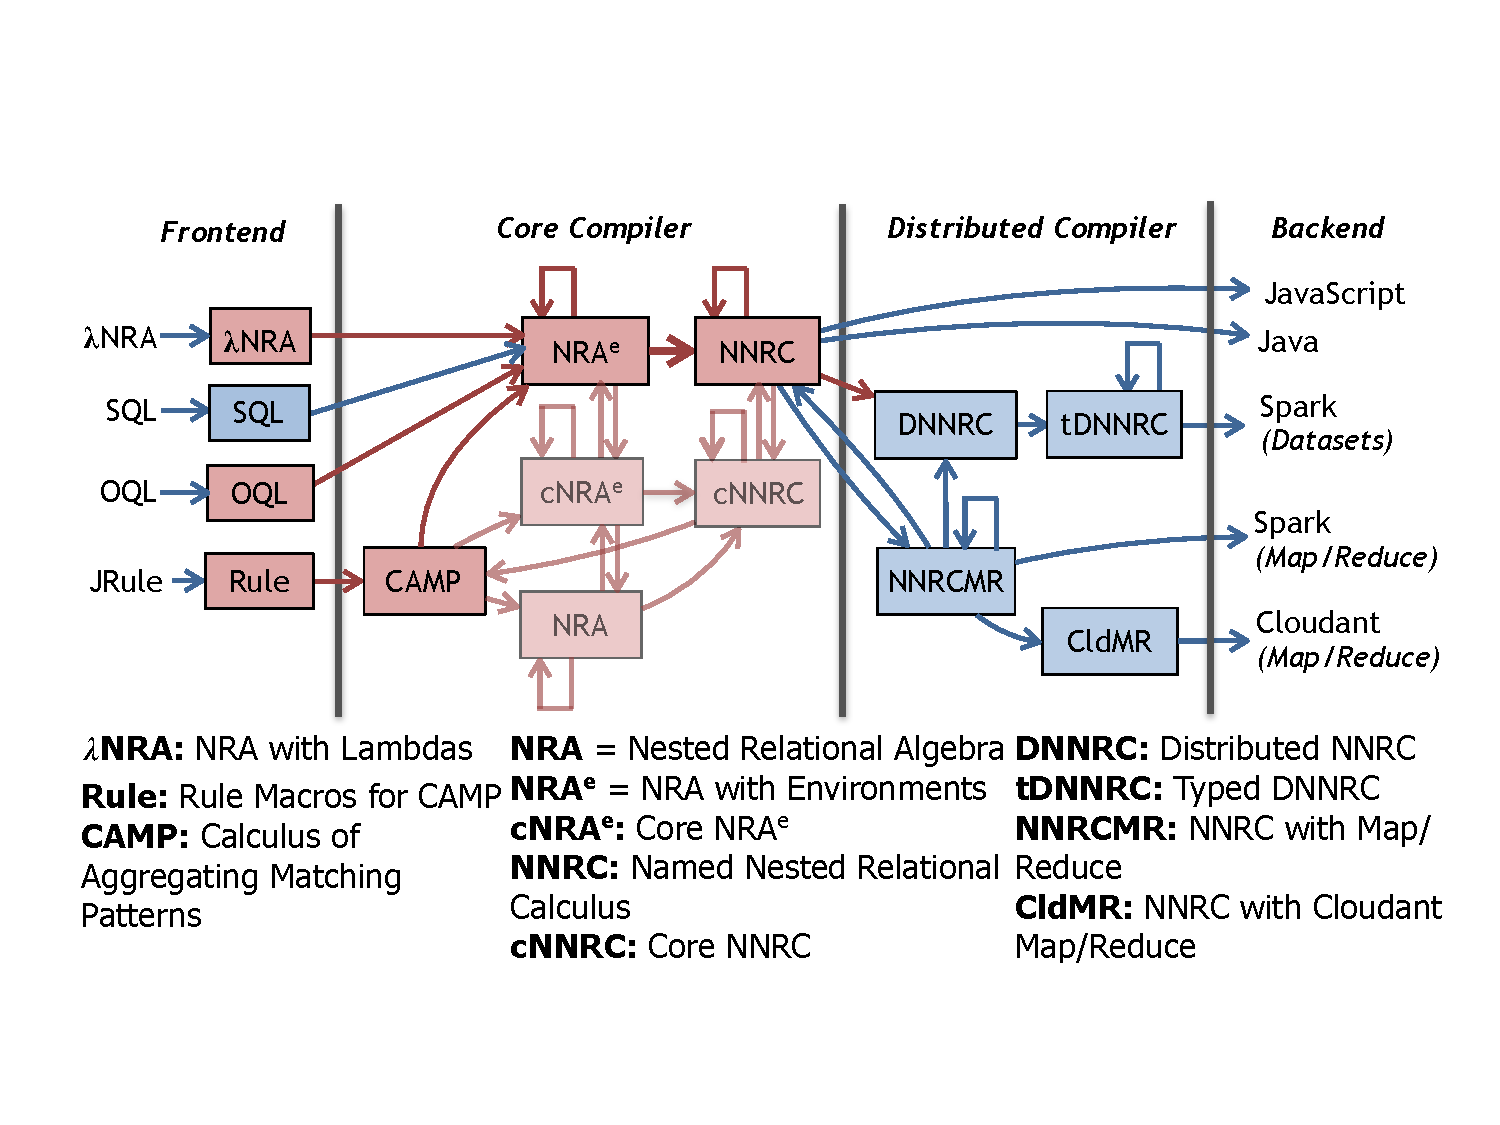
\includegraphics[width=0.48\textwidth]{qcert-pipeline.pdf}}
  \caption{\label{fig:architecture}Q*cert compiler architecture.}
\end{figure}

From a front-end perspective, the system includes a parser for OQL and
\NRALambda. JRules and SQL support rely on existing Java parsers for
those languages, which pass an AST to the compiler encoded as an
S-expression. The named nested relational calculus (NNRC) is the
gateway to the backend part of the compiler. It is directly used to
generate code for Java and JavaScript, while code generation for Spark
and Cloudant rely on additional intermediate representations (DNNRC
models distributed computation with Spark Datasets, NNRCMR models
map/reduce, and CldMR models Cloudant-specific map/reduce).

\paragraph*{Data model and type system}

In order to focus on the novel features of \NRAEnv, this paper uses a
simple data model of complex values with bags and records, and omits
the treatment of types. This is far from enough for practical
languages. For instance, OQL and JRules support class hierarchies, and all
our languages require support for null values, date comparisons, and
arithmetic. The implementation supports a rich data model that
includes a notion of objects as well as sum types in a way similar
to~\cite{GiorgidzeGUW12,WF2016}. The compiler specification and
correctness proofs are done over that richer data model and type
system. It is important to recall that type correctness is used
pervasively as a pre-condition for algebraic rewrites and rely on type
checking and type soundness proofs for the intermediate languages.

To handle additional data types (e.g., dates), and provide some
modularity, the mechanization is parameterized over a notion of
``foreign'' types and operators. From a Coq perspective, those are
\emph{axioms} that are assumed by the proof system. A set of axioms
for each foreign type typically includes semantics and typing
judgments, with correctness
properties\,\coqdef{Basic.ForeignRuntime}{}. When the compiler is
extracted, an \emph{implementation} of those axioms as regular code
must be provided. Note that this choice represents a trade-off, since
Coq cannot ensure the correctness of that part of the implementation.

\paragraph*{Optimizer}

Most of the formal treatment of the paper uses algebraic equivalences
to convey optimizations. As we mentioned in the introduction, those
are used as part of the proof of correctness for the optimizer
itself. These optimizations are written as individual pattern-match
based transformations (with side conditions as needed), each of which
is proven to preserve semantics (and typing as appropriate).

The optimization infrastructure is parameterized by a list of rewrites
and a cost function. All possible rewrites are applied through a
depth-first AST traversal and optimization proceeds as long as the
cost is decreasing.
%
Despite being simple by traditional databases standards, the optimizer
includes on the order of a hundred rewrites. The cost is currently
based on the size and depth of the query which means there is a lot of
room for improvements on that part of the implementation. Coq does not
introduce specific limitations as to the complexity of the optimizer,
which could use a search space and more complex cost model.

Finally, we have made some efforts to ensure that adding new
optimizations is relatively straightforward. As shown in the
introduction, each rewrite can be programmed and proved individually.
The infrastructure provides a tactic that helps with this, in order to
automatically reduce the full proof to a proof of the individual
type-directed rewrite.

\paragraph*{Support for other languages}

Our current compiler uses well-known database representations which
means it can easily be used to investigate or validate novel
optimizations for other use cases, as we have done for CAMP. The
amount of work required for adding a new language to the compiler
depends on the nature of the language. Q*cert makes a few important
assumptions: one is a data model based on nested relations, the other
is that type checking is assumed in most of the optimizer support. As
a result, the compiler should be a good match for Spark~(which we
partially support), Pig~Latin~\cite{OlstonRSKT08}, or JSON languages
such as Jaql~\cite{BeyerEGBEKOS11-full}. Additional work on typing for
semi-structured data would make languages such as
JSONiq~\cite{florescu2013jsoniq} or SQL++~\cite{OngPV14} interesting
next steps. Languages such as XQuery would require significant changes
to the compiler because of the complexity of the XML data model.

\paragraph*{Thoughts on Coq}

Coq is a functional programming language that fits well the task of
writing compilers. Proofs can be added gradually, extraction is
robust, and the code generated benefits from the good quality of the
OCaml compiler, both in terms of stability and performances. The
current performance bottlenecks in our implementation are in the
optimizers, which can lead to an exponential number of iterations over
the tree. However, it should be possible to use memoization techniques
to improve performances~\cite{braibant2014implementing}.

One of the pleasant surprises of our experience has been the
versatility of Coq, which we feel could be used to tackle a range of
database problems. For instance, similar techniques could be used for:
the specification of a query language after the fact or during
development (for documentation and prototyping), ensuring the
correctness of complex algorithms (e.g., view maintenance), or
building an end-to-end verified compiler. This last scenario
would certainly be a large undertaking and would require addressing
integration issues with a real database engine.

%%% Local Variables:
%%% TeX-master: "main"
%%% End:

\section{Related Work}
\label{sec:related}

There has been renewed interest in the formal verification of
database systems or query
languages~\cite{BenzakenCD14,CheneyU11,malecha2015,MalechaMSW10,ShinnarSH15}. So
far, much of the work has focused on
formalization~\cite{BenzakenCD14,CheneyU11,ShinnarSH15} or on
evaluating challenges involved in
mechanization~\cite{MalechaMSW10}. The closest related work is that of
Cherniack and Zdonik~\cite{cherniack1996rule,CherniackZ98}, which
focused on the formal specification of rule-based query optimizers and
used the Larch~\cite{Larch89} theorem prover to verify
correctness. Our work extends that approach in two ways: (i) we
describe an alternative combinator-based algebra with built-in support
for environments and (ii) we leverage recent advances in theorem
proving technology to specify a much larger part of the query
compiler.

How to best deal with variables and environments in algebraic
compilers has received relatively little attention. For SPJ
(Select-Project-Join) queries, variables can be eliminated at
translation time and equivalences can be simply defined for a given
static environment~\cite{aho1979efficient}. For query languages over
complex or nested data, reification of the environment as a record is
appealing in that existing relational techniques can be readily
applied. This idea has notably been used in algebraic compilers for
query languages over nested or graph data such as OQL~\cite{CluetM93}
and XQuery~\cite{MayHM04,re2006complete}. Full reification enables
relational optimizations, but can result in large or highly nested
plans in those languages as well. The algebra from~\cite{CluetM93}
does combine environments and reification, but assumes that
environments are fixed for the purpose of defining plan equivalence.

Dealing with bindings is also important for the formalization of
programming languages. The POPLmark
challenge~\cite{AydemirBFFPSVWWZ05} has helped spur an assortment of
techniques for representing and reasoning about bindings.  These are
all focused on traditional bindings, as introduced by functions.  Our
work uses explicit reified environments instead. It enables support
for the standard shadowing semantics for occurrences of a variable
while also supporting unification semantics, where the value of the
variable added to the environment has to be compatible with 
previous occurrences.

%%% Local Variables:
%%% TeX-master: "main"
%%% End:

\section{Conclusion}
\label{sec:conclusion}

This paper introduced \NRAEnv, the Nested Relational Algebra with
Environments, which provides the foundation for a formally verified
query compiler written using the Coq proof assistant. \NRAEnv extends
a combinators-based nested relational algebra with explicit
environment support in a way that facilitates the specification and
verification of algebraic rewrites. A lifting theorem shows that all
existing NRA optimizations also apply to \NRAEnv. We showed how the
resulting compiler can be used for both traditional queries and for a
query DSL in the context of a rules language. 

Theorem proving techniques have greatly matured in recent years, and
we feel that their application to databases could prove useful in a number
of ways (for specification, prototyping, or to provide correctness
guarantees in scenarios where security or privacy are important). We
are currently working on further improvements to our compiler
infrastructure, notably to the optimizer and backend, in order to
support code-generation for distributed query plans.

%%% Local Variables:
%%% TeX-master: "main"
%%% End:


\paragraph*{Acknowledgments} We would like to thank the anonymous
reviewers for their comments and suggestions which greatly helped us
improve the content and presentation of this work. We also thank
Guillaume Baudart, Stefan Fehrenbach, and Erik Wittern for their
feedback on earlier drafts.
%
Finally, we send this \text{\href{http://lucy-n.org/papers/Plateau-These-2010.pdf\#page=49}{\fleur}} to Florence Plateau.

\bibliographystyle{abbrv}
\bibliography{main}

\appendix

\section{CAMP}
\label{sec:CAMP}

Section~\ref{sec:rules} discussed the CAMP calculus, which was
originally described in~\cite{ShinnarSH15} as a useful intermediate
language for compiling rule-based languages.  Section~\ref{sec:rules}
reported on the results of translating and optimizing CAMP through
\NRAEnv.  In this appendix, we formalize the translation from CAMP to
\NRAEnv, and present some important NRA optimizations that help
simplify the resulting \NRAEnv.

The paper that introduced the CAMP calculus presents a translation
into NRA in Figure~10 of \cite{ShinnarSH15}. This required encoding
the input as a record with two components $D$ and $E$ representing the
current data and environment.  \NRAEnv avoids the need for such an
encoding, as the CAMP environment can be directly represented using
the \NRAEnv environment.  Figure~\ref{fig:tonraenv-trans} presents the
full translation from CAMP to \NRAEnv (on the right). For comparison,
the original translation from~\cite{ShinnarSH15} is presented in
parallel (on the left).

Consider for example the translation of $\rmap{p}$. When we go to
\NRAEnv, the translation produces a corresponding map in \NRAEnv, and
uses a flattening to account for the fact that the result of
translating~$p$ will return a collection:
$$
\pton{\rmap{p} } = \left\{\opflatten\left(\qmap{\ntop{p}}{\qID}\right)\right\}
$$
When we go to NRA, in addition to the flattening, the input must be manipulated
to iterate on the data part and keep
the environment. The translation function is:
$$
\begin{array}{l}
\hspace*{-0.1cm}\pton{\rmap{p}} =
\\
  \left\{\opflatten\left(\qmap{\ntop{p}}{\quntwo{T}{D}{\{[E:\qID.E]\opconcat[T:\qID.D]\}}}\right)\right\}
\end{array}
$$
where $\quntwo{A}{B}{q}$ is the unnest operator from
Section~\ref{sec:nraenv:nra}.

In addition to the \NRAEnv\ specific optimizations presented
in Figure~\ref{tab:rewrites}, many standard NRA optimizations are useful for
optimizing translated CAMP.  Figure~\ref{tab:rewrites-nra} presents a
number of these optimizations, which serve to eliminate inefficiencies introduced either by
the structure of the CAMP language or naive translation.  Similarly,
Figure~\ref{tab:rewrites-nraenv} presents more complex \NRAEnv\
optimizations that target common patterns produced by compilation
from CAMP.
\balance

\begin{figure*}[b]
  \centering
  \[\begin{array}{>{\color{darkergray}}lcccll}
\multicolumn{1}{c}{\color{darkergray}\text{NRA}} && \text{CAMP} && \multicolumn{1}{c}{\text{\NRAEnv}}\\
\hline
\{d\}&=&\pton{d}&=&\{d\}\\
\qmap{\opunop \qID}{\pton{p}}&=&\pton{\opunop p}&=&\qmap{\oplus \qID}{\pton{p}}\\
\Big(\chi\!_{\left\langle{\qID.T_1 \opbinop \qID.T_2}\right\rangle}&=&\pton{p_1 \opbinop p_2}&=&\Big(\chi\!_{\left\langle{\qID.T_1 \opbinop \qID.T_2}\right\rangle}\\
\qquad\qmap{[T_1:\qID]}{\ntop{p_1}}\times \qmap{[T_2:\qID]}{\ntop{p_2}}\Big)&&&&\qquad\qmap{[T_1:\qID]}{\ntop{p_1}}\times \qmap{[T_2:\qID]}{\ntop{p_2}}\Big)\\
\Big\{\opflatten\big(\chi_{\left\langle{\ntop{p}}\right\rangle}&=&\pton{\rmap{p} }&=&\left\{\opflatten\left(\qmap{\ntop{p}}{\qID}\right)\right\}\\
\multicolumn{2}{l}{\color{darkergray}\qquad\left({\quntwo{T}{D}{\{[E:\qID.E]*[T:\qID.D]\}}}\right)\big))\Big\}}\\
\qmap{[\,]}{\qselect{\qID}{\pton{p}}}&=&\pton{\rassert{p}}&=&\qmap{[\,]}{\qselect{\qID}{\pton{p}}}\\
\ntop{p_1}\qor\ntop{p_2}&=&\pton{ p_1\ror p_2}&=&\pton{p_1}\qor\pton{p_2}\\
\{\qID.D\}&=&\pton{\rit}&=&\{\qID\}\\
\opflatten\Big(\chi\!_{\left\langle\pton{p_2}\right\rangle}&=&\pton{\rleti{p_1}{p_2}}&=&\opflatten\left(\qmap{\ntop{p_2}}{\pton{p_1}}\right)\\
\multicolumn{2}{l}{\color{darkergray}\qquad \left({\quntwo{T}{D}{\{[E:\qID.E]*[T:\pton{p_1}]\}}}\right)\Big)}\\
\{\qID.E\}&=&\pton{\renv}&=&\{\qENV\}\\
\opflatten\Big(\chi\!_{\left\langle\pton{p_2}\right\rangle}(&=&\pton{\rlete{p_1}{p_2}}&=&\opflatten\Big(\qmapenv{\ntop{p_2}} \circ^e \opflatten\left(\qmap{\qID \opmergeconcat \qENV}{\ntop{p_1}}\right)\Big)\\
\multicolumn{4}{l}{\color{darkergray}\qquad\qquad\quad\chi\!_{\left\langle[E:\qID.E_2]*[D:\qID.D]\right\rangle}(}\\
\multicolumn{4}{l}{\color{darkergray}\qquad\qquad\qquad\quntwoop{T_2}{E_2}
(
\chi\!_{\left\langle\qID*[T_2:\qID.E+\qID.E_1]\right\rangle}
(}\\
\multicolumn{4}{l}{\color{darkergray}\qquad\qquad\qquad\quad\quntwo{T_1}{E_1}
{
 \{
\qID*[T_1:\pton{p_1}]
\}
}
)
)))\Big)}
\end{array}\]
\caption{From CAMP {\color{darkergray}to NRA\,\coqdef{Translation.CAMPtoNRA}{nra_of_pat} and} \NRAEnv\,\coqdef{Translation.CAMPtoNRAEnv}{nraenv_of_pat} \fbox{\(\pton{p} = q\)}}
  \label{fig:tonraenv-trans}
\end{figure*}

\begin{figure*}[hb]
  \begin{minipage}{0.49\linewidth}
    \centering
    \[\begin{array}{r@{\ }c@{\ }ll}
        [ a : q ].a & \Rightarrow & q
        & \coqdef{NRAEnv.Optim.TNRAEnvRewrite}{tdot_over_rec_arrow}
        \\
        (q_1 \opconcat [ a_2 : q_2 ]).a_2 & \Rightarrow & q_2
        & \coqdef{NRAEnv.Optim.TNRAEnvRewrite}{tdot_over_concat_eq_r_arrow}
        \\
        \mbox{if~} a_1 \neq a_2,\ (q \opconcat [ a_2 : q_2 ]).a_1 & \Rightarrow & q.a_1
        & \coqdef{NRAEnv.Optim.TNRAEnvRewrite}{tdot_over_concat_neq_r_arrow}
        \\
        \mbox{if~} a_1 \neq a_2,\ ([ a_1 : q_1 ] \opconcat q).a_2 & \Rightarrow & q.a_2
        & \coqdef{NRAEnv.Optim.TNRAEnvRewrite}{tdot_over_concat_neq_l_arrow}
        \\
        \,[\,] \opmergeconcat q & \Rightarrow & \{ q \}
        & \coqdef{NRAEnv.Optim.TNRAEnvRewrite}{tmerge_empty_record_l_arrow}
        \\
        q \opmergeconcat [\,] & \Rightarrow & \{ q \}
        & \coqdef{NRAEnv.Optim.TNRAEnvRewrite}{tmerge_empty_record_r_arrow}
        \\
        \{ [ a_1 : q_1 ] \} \times \{ [ a_2 : q_2 ] \} & \Rightarrow & \{ [ a_1 : q_1] \opconcat [ a_2 : q_2 ] \}
        & \coqdef{NRAEnv.Optim.TNRAEnvRewrite}{tproduct_singletons_arrow}
        \\
        \qID \circ q & \Rightarrow & q
        & \coqdef{NRAEnv.Optim.TNRAEnvRewrite}{tapp_over_id_l_arrow}
        \\
        (\opunop(q_1)) \circ q_2 & \Rightarrow & \opunop(q_1 \circ q_2)
        & \coqdef{NRAEnv.Optim.TNRAEnvRewrite}{tapp_over_unop_arrow}
        \\
        (q_2 \opbinop q_1) \circ q & \Rightarrow & (q_2 \circ q) \opbinop (q_1 \circ q)
        & \coqdef{NRAEnv.Optim.TNRAEnvRewrite}{tapp_over_binop_arrow}
        \\
        \mbox{if~} \igni{q_1},\ q_1 \circ q_2 & \Rightarrow& q_1
        & \coqdef{NRAEnv.Optim.TNRAEnvRewrite}{tapp_over_ignoreid_arrow}
        \\
      \end{array}
     \]
  \end{minipage}
  \begin{minipage}{0.50\linewidth}
    \centering
    \[\begin{array}{r@{\ }c@{\ }ll}
        \qmap{q_1}{q_2} \circ q & \Rightarrow & \qmap{q_1}{q_2 \circ q}
        & \coqdef{NRAEnv.Optim.TNRAEnvRewrite}{tapp_over_map_arrow}
        \\
        \opflatten(\qmap{\qmap{\{ q_3 \}}{q_1}}{q_2}) & \Rightarrow & \qmap{\{ q_3 \}}{\opflatten(\qmap{q_1}{q_2})}
        & \coqdef{NRAEnv.Optim.TNRAEnvRewrite}{tdouble_flatten_map_coll_arrow}
        \\
        \qmap{p_1}{\opflatten(p_2)} & \Rightarrow & \opflatten(\qmap{\qmap{p_1}{\qID}}{p_2})
        & \coqdef{NRAEnv.Optim.TNRAEnvRewrite}{tmap_over_flatten}
        \\
        \qmap{p_1}{\opflatten(\qmap{p_2}{p_3})} & \Rightarrow & \opflatten(\qmap{\qmap{p_1}{p_2}}{p_3})
        & \coqdef{NRAEnv.Optim.TNRAEnvRewrite}{tmap_over_flatten_map}
        \\
        \opflatten(\{ q \}) & \Rightarrow & q
        & \coqdef{NRAEnv.Optim.TNRAEnvRewrite}{tenvflatten_coll_arrow}
        \\
        \opflatten(\qmap{\{ q_1 \}}{q_2}) & \Rightarrow & \qmap{q_1}{q_2}
        & \coqdef{NRAEnv.Optim.TNRAEnvRewrite}{tenvflatten_map_coll_arrow}
        \\
        \qmap{\qID}{q} & \Rightarrow & q
        & \coqdef{NRAEnv.Optim.TNRAEnvRewrite}{tenvmap_into_id_arrow}
        \\
        \qmap{q_1}{\qmap{q_2}{q}} & \Rightarrow & \qmap{q_1 \circ q_2}{q}
        & \coqdef{NRAEnv.Optim.TNRAEnvRewrite}{tenvmap_map_compose_arrow}
        \\
        \qmap{q_1}{\{ q_2 \}} & \Rightarrow & \{ q_1 \circ q_2 \}
        & \coqdef{NRAEnv.Optim.TNRAEnvRewrite}{tenvmap_singleton_arrow}
        \\
        \qmap{q_2}{\qselect{q_1}{\{ q \}}} & \Rightarrow & \qmap{q_2 \circ q}{\qselect{q_1 \circ q}{\{ \qID \}}}
        & \coqdef{NRAEnv.Optim.TNRAEnvRewrite}{tmap_full_over_select_arrow}
        \\
      \end{array}
     \]
  \end{minipage}
 \vspace*{1.5mm}
  \caption{NRA rewrites for CAMP.}
  \label{tab:rewrites-nra}
\end{figure*}

\begin{figure*}[ht]
  \begin{minipage}{0.99\linewidth}
    \centering
    \[\begin{array}{r@{\ }c@{\ }ll}
    \opflatten(\qmapenv{\qmap{\qENV}{\qselect{q_1}{\{ \qID \}}}}) \circ^e \qmap{\qENV}{\qselect{q_2}{\{ \qID \}}} & \Rightarrow&\qmap{\qENV}{\qselect{q_1}{\qselect{q_2}{\{ \qID \}}}}
    & \coqdef{NRAEnv.Optim.TNRAEnvRewrite}{tcompose_selects_in_mapenv_arrow}
    \\
    (\qmapenv{q}) \circ^e (\qENV \opmergeconcat [ a : \qID ]) & \Rightarrow& \qmap{(q \circ \qENV.a) \circ^e \qID}{\qENV \opmergeconcat [ a : \qID ]}
    & \coqdef{NRAEnv.Optim.TNRAEnvRewrite}{tappenv_mapenv_to_map_arrow}
    \\
    \opflatten(\qmapenv{q}) \circ^e (\qENV \opmergeconcat [ a : \qID ]) & \Rightarrow& \opflatten(\qmap{( q \circ \qENV.a ) \circ^e \qID}{\qENV \opmergeconcat [ a : \qID ]})
    & \coqdef{NRAEnv.Optim.TNRAEnvRewrite}{tappenv_flatten_mapenv_to_map_arrow}
    \\
    \qmap{\qENV \opmergeconcat \qID}{\qselect{q_1}{\qENV \opmergeconcat q_2}} & \Rightarrow& \qmap{\{ \qID \}}{\qselect{q_1}{\qENV \opmergeconcat q_2}}
    & \coqdef{NRAEnv.Optim.TNRAEnvRewrite}{tflip_env6_arrow}
    \end{array}\]
  \end{minipage}  \vspace*{1.5mm}
  \caption{\NRAEnv\ rewrites for CAMP.}
  \label{tab:rewrites-nraenv}
\end{figure*}

%%% Local Variables:
%%% TeX-master: "main"
%%% End:


\end{document}

%%% Local Variables:
%%% TeX-master: "main"
%%% End:
